\let\textcircled=\pgftextcircled
\chapter{Metastable state selection for Hidden Markov Models}
\label{chap:hmm}

\section{Introduction}
The previous chapter demonstrated optimizing the discretization of MD trajectories into discrete states for analysis using Markov state models. A large number of microstates in the optimized model and the sensitivity tests ($110 < n < 310$) were required in the trade-off between accuracy and statistical certainty. While this produces the most accurate picture possible given the data, to gain a more intuitive and manageable picture the MSM must be coarse grained into a smaller number of macrostates. There have been a large number of different methods proposed for accomplishing this task. One of the first was Perron Cluster Cluster Analysis (PCCA, and it's more numerically robust successor PCCA+)  []  uses the sign structure of the eigenvectors to lump microstates into metastable macrostates. Many other schemes have been proposed using mechanisms other than metastability and addressing different problems. For example HNEG uses the Nystr\:{o}m method to emphasize well-sampled states in coarse graining, overcoming the problem of under-sampled microstates giving rise to spurious distinct macrostates.  BACE uses Bayes factors to decide whether two microstates should be separate or lumped together in a macrostate. Many other methods exist [MPP, CatProcess, OptDimRed, Renorm] and have been quantitatively compared in []. One of the most popular methods is Hidden Markov Models []. HMMs are a well developed statistical tool, well understood and with a number of attractive properties for protein dynamics. First, they maintain the experimentally observed metastability of protein dynamics, not in the observed microstate conformations but in a set of hidden states. This drops the restriction of Markovianity in the observed states. Second, they have been shown to be robust to poor discretisations of the state space and third, observables are easily calculated from the model parameters. 

In all coarse-graining methods the number of macrostates must be stipulated as a hyper-parameter. For PCCA(+) and HMMs it is usual to inspect the eigenvalue spectrum of the MSM and look for gaps in successive eigenvalues or implied timescales. The motivation behind this is that these gaps define a separation of timescales into slow relaxation processes dominate the long term macrostate evolution. The problem with this method is that in practice insufficient sampling leads to gaps which statistically indistinguishable.  Other methods utilise different criteria which suffer from problems of subjectivity,  see the previous referenced papers and \cite{bowmanQuantitativeComparisonAlternative2013} for a discussion.  

Bayes factors [] have been proposed as a method of not only choosing the number of macrostates for a coarse graining method but of quantitatively comparing arbitrary coarse-graining schemes. The Bayes factor of two models, $M_{1}$ and $M_{2}$ is equal to the ratio of the integrated likelihood of the data, $D$, given the model: 

\begin{equation}
\operatorname{BF} = \frac{P(D|M_1)}{P(D|M_2)}
\end{equation}

If the prior probability of the models are equal, i.e. $P(M_1)=P(M_2)$, then by Bayes law the BF is equal to the ratio of the probabilities of each model given the data $P(M|D)$. If $BF > 1$ then model $1$ is favoured and vice versa. In the case of coarse graining Markov models for protein dynamics, the data are the discrete microstate trajectories $D = (s_1, s_2, ..., s_T)= \{s_t\}$, and the model is the coarse graining definition which includes the number of macrostates. If the  

HMMs are a type of finite mixture model \cite{mclachlanFiniteMixtureModels2000}, where the observed data are supposed to be generated by a collection of hidden or latent states, mixed in some proportion. An HMM is differentiated from, say a Gaussian mixture model, by virtue of the Markov relation between the hidden states. A general finite mixture model is defined as: 

\begin{equation}
    f(s_{t}) = \sum_{i=1}^{g}\tilde{pi}_{i} f_{i}(s_{t})
\end{equation}

Here $s_{t}$ are the observations, indexed by $t$; $f()$ is the distribution of the observations; $\tilde{\pi}$ are the mixing proportions of the $g$ hidden states; and $f_{i}$ is the distribution of the data  conditional on the hidden state $i$. In the context of biomolecular Markov models, $\{s_t\}$ the $n$ observed microstates at time $t$. $f(s_{t})$ is a categorical distribution over the  microstates with parameters $\pi_1, \pi_2, ... \pi_n$ i.e. whose parameters constitute the stationary distribution over the microstates. The parameters  $\tilde{pi}_{1},\tilde{pi}_{2}, ..., \tilde{pi}_{g}$ are the stationary distribution of the metastable states. In keeping with notation in \cite{noeProjectedHiddenMarkov2013a} the tilde over the symbol refers to the hidden states.  $f_{i}(s_t)$ are categorical distributions corresponding to the rows of the emission matrix, i.e. $f_{i}(s_t)= f_{i}(s_t; p^{i}_1, p^{i}_2, ..., p^{i}_n)$ so that for a hidden state $h$ and observed state $s$,$P(s=j|h=i) = p^{i}_{j}$. The extra Markov constraint links the evolution of the hidden states via $\tilde{\mathbf{T}}(\tau)$. The parameters estimated in fitting a HMM are those of the emission matrix, $p^{i}_{j}$, and the hidden state transition matrix, $\tilde{\mathbf{T}}$.

There are a number of different approaches to selecting the number of hidden states in mixture models: 
\begin{enumerate}
    \item \emph{Likelihood ratio test (LRT):} The use of the likelihood ratio test for mixture models is still debated \cite{mclachlanFiniteMixtureModels2000}\cite{celeuxSelectingHiddenMarkov2008}\cite{cappe2006inference}  due the validity of the conditions under which the asymptotic null distribution has the standard $\chi^{2}$ distribution. The LRT will not be considered further here. 
    \item \emph{Cross-validated likelihood:} The cross-validated likelihood has been used in both mixture models \cite{smythModelSelectionProbabilistic2000} and for hidden Markov models \cite{celeuxSelectingHiddenMarkov2008}. 
    \item \emph{Information criteria:} There are a number of different information criteria, see chapter 6 of \cite{mclachlanFiniteMixtureModels2000} for an overview. They fall into three broad categories:
    \begin{enumerate}
        \item Kullback-Leibler [] divergence minimizers: e.g. the Akaike Information Criterion []. These aim to minimize the divergence between the true distribution and the model distribution as measured by the Kullback-Leibler divergence. 
        \item Bayesian model selectors: these select models based on the approximations to the posterior odds of two competing models or Bayes Factor [], e.g. the Bayesian information criterion [].  
        \item Classification likelihood selectors: just as the likelihood is a measure of the goodness-of-fit of a given model to the \emph{observed} data $\mathbf{s}_t$, the classification (or complete data) likelihood [] is the goodness-of-fit to the observed \emph{and hidden} data, $(\mathbf{s}_t, \mathbf{h}_t)$, e.g. the Integrated Classification likelihood criterion, ICL [].
    \end{enumerate}
\end{enumerate}
 
 In addition to the model selection techniques from the mixture model literature, there are a number of other techniques which have been developed within the biomolecular simulation community. The authors of \cite{bacalladoBayesianComparisonMarkov2009a}, developed a fully Bayesian computation of Bayes factors, with priors respecting detailed balance, to compare arbitrary coarse graining methods (not just HMMs), which can include selecting the number of hidden states \cite{bowmanQuantitativeComparisonAlternative2013}. A more common method is to look for the largest gap in the eigenvalue spectrum of the observed transition matrix, as suggested in numerous places [pcca]\cite{mcgibbonVariationalCrossvalidationSlow2015}\cite{prinzMarkovModelsMolecular2011} and as performed in chapter \ref{chap:aadh} for the reference MSM of AADH. 
 
Once a number of hidden states has been selected, the model must be validated within statistical uncertainty. The methods for quantifying uncertainty of MSMs and HMMs estimated using maximum likelihood using confidence intervals are not appropriate using the sliding window method for constructing the count matrix. Bootstrapping methods are possible but the more straight forward method is to quantify the uncertainty using probability with Bayesian estimation. In order to estimate a Bayesian model, once the prior has been specified, is to sample independent MCMC chains from the posterior distribution and check for convergence in parameter estimates.  This is performed by checking for a lack of auto-correlation in the chains and through convergence statistics such as the Gelman-Rubin statistic. If a Bayesian model can be converged then the Chapman-Kolmogorov test and implied timescale plots can be used to the check the consistency of the model with the data and to test the Markov assumption to within statistical uncertainty. 

This chapter investigates the use of information criteria and likelihood based methods for choosing the number of metastable states in addition to Bayesian model validation. It will use the four well Prinz potential specified at a series of lag times to provide a well understood system to investigate the cross-validated log likelihood, AIC, BIC and ICL selection criteria. Once the behaviour of these indicators is understood, these techniques will be applied to the case of AADH to determine the number of metastable states in the discrete models estimated in  chapter \ref{chap:msm}. The structure is as follows: in section \ref{sec:hmm_methods} the Prinz potential, and the model selection criteria will be explained; section \ref{sec:hmm_results} discusses the results for both the Prinz potential and AADH; section xxx concludes with discussions for further work. 


\section{Methods} \label{sec:hmm_methods}
\subsection{Data}

This work evaluates model selection techniques for Hidden Markov Models on two systems: the Prinz potential and AADH. 

\subsubsection{Prinz potential}
\begin{figure}
    \centering
    \mycaption{The Prinz potential. Panel (a) shows the potential $V(x)$ in blue and the stationary distribution $\pi(x)$ in orange. Panel (b) shows the first $12$ eigenvalues (evaluated with $\tau=5$ time-steps). Panel (c) shows the implied timescales (in units of the time-step $\Delta t=0.001$) in blue and the values of $\tau = 5, 8, 37, 94, 484$ time-steps used in the model selection  experiments as black dashed lines.}
    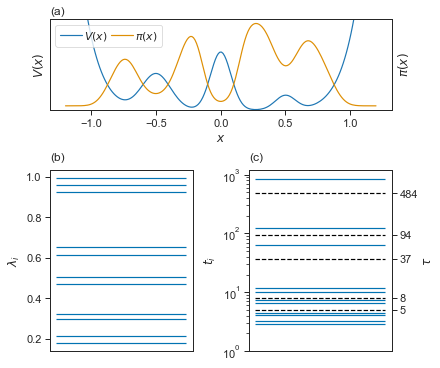
\includegraphics[height=0.4\textheight]{chapters/hmm_selection/figures/prinz_pot.png}
    \label{fig:prinz}
\end{figure}

The Prinz potential \cite{prinzMarkovModelsMolecular2011} is a four well potential shown in figure \ref{fig:prinz}. The potential is given by: 
\begin{equation}\label{eqn:prinz_pot}
       V(x) = 4\left(x^8 + 0.8 \exp{\left(-80 x^2\right)} + 0.2 \exp{\left(-80 (x-0.5)^2\right)} + 0.5\exp{\left(-40 (x+0.5)^2\right)}\right).
\end{equation}
Exact eigenvalues and trajectories of simulated Brownian motion were calculated using code from MSMBuilder \cite{beauchampMSMBuilder2ModelingConformational2011} version 3.9.0.  The simulations solved the following stochastic differential equation: 

\begin{equation}\label{eqn:prinz_dynamics}
    \frac{\mathrm{d}x_t}{\mathrm{d}t} = -\frac{\mathrm{d}V(x)}{\mathrm{d}x} + \sqrt{2D} * R(t)
\end{equation}

with $D = 1000$, and $R\sim \mathcal{N}(0, 1)$, $\mathrm{Cov}\left[R(t), R(t^{\prime})\right]=\delta_{t, t^{\prime}}$. The time-step used was $\Delta t = 0.001$.  Each trajectory was initiated from a random draw of the stationary distribution and was twice the longest relaxation process timescale, i.e. $2\times 844=1688$ time-steps long. The trajectories were clustered into $n = \left\lfloor\sqrt{100\times 1688}\right\rfloor =410$ discrete states using k-means clustering \cite{friedman2001elements}. This number of states was based on the heuristic described in \cite{husicWardClusteringImproves2017a}.


\subsubsection{AADH}
The data for the AADH system comprise the MSMs and associated discrete trajectories of the base case and three sensitivities described in chapter \ref{chap:msm} section \ref{subsubsec:sensitivity_analysis}. The model specifications are tabulated here in table \ref{tab:aadh_final_msm_specs}. 

\begin{table}
    \centering
    \mycaption{Markov lag time and MSM hyper-parameters. These MSMs and the associated discrete trajectories form the data for the HMM coarse graining.}
    \begin{tabular}{|l|l|l|l|l|}
        \hline
        Parameter & Base case & Sensitivity 1 & Sensitivity 2 & Sensitivity 3 \\
        \hline\hline
        Markov lag time, $\tau(\textrm{MSM})$ & \SI{2}{\nano\second} &  \SI{20}{\nano\second}& \SI{2}{\nano\second}& \SI{2}{\nano\second} \\
        Feature, $\chi$ & $(\phi, \psi, \chi)$ & $(\phi, \psi, \chi)$ & $|\mathbf{r}_{1}-\mathbf{r}_2|$ & $(\phi, \psi, \chi)$ \\
        TICA lag time, $\tau$ & \SI{10}{\nano\second} & \SI{10}{\nano\second}&\SI{1}{\nano\second} &\SI{85}{\nano\second} \\
        TICA components, $m$ & $2$ & $2$ & $2$ & $2$ \\
        Cluster centres, $n$ & $310$ & $310$ & $110$ & $310$ \\
        \hline
    \end{tabular}
    \label{tab:aadh_final_msm_specs}
\end{table}

\subsection{Model selection criteria}

This work will compare the use of the following model selection techniques for coarse graining MSMs using HMMs.  

\subsubsection{The Akaike Information Criterion, AIC}. The AIC is defined as:

\begin{equation}
    \operatorname{AIC} = -2\left(\log{L\left(\{s_t\}|\hat{\theta}\right)} - d\right)
\end{equation}

Where $\hat{\theta}$ is shorthand for the maximum likelihood estimates of the model parameters, i.e. $\tilde{\mathbf{T}}, \mathbf{E}$. So $L(\{s_t\}|\theta)$ is the likelihood of the observed data $\{s_t\}$ given the hidden Markov model parameters,  and $d$ is the degrees of freedom in the model. For a reversible hidden Markov model with $g$ hidden states and $n$ observed states  $d = \sfrac{1}{2}g(g-1) + (g-1) + g(n-1)$ \cite{trendelkamp-schroerEstimationUncertaintyReversible2015b}. The origin of the two terms in parentheses arises from the approximation of the KL divergence using the empirical density instead of the true underlying density (the log-likelihood term) and a bias correction (the $d$ term). The $-2$ is there to make an equivalence with Mallows $C_p$ \cite{friedman2001elements}. The selected model is the one which has the smallest AIC or in other words, the model which has the smallest KL divergence relative to the true data generating process. 

\subsubsection{The cross-validated log-likelihood, CVLL}. The cross-validated log-likelihood also approximates the KL-divergence \cite{celeuxSelectingHiddenMarkov2008}. The CVLL is calculated in the following way: 
\begin{enumerate}
    \item The observed trajectories are split into $N$ training $\mathbf{s}^{i}$ and test $\mathbf{s}^{-i}$, $i = 1, ..., N$ sets using 50:50 shuffle-split, as described in chapter \ref{chap:msm} section \ref{sec:methods}. 
    \item For each $i$, fit a HMM using the training data $\mathbf{s}^{i}$. 
    \item Calculate the likelihood of the test data $\mathbf{s}^{-i}$, given the HMM parameters estimated on the training data, $L(\mathbf{s}^{-i}|\hat{\theta}^{i})$ using the forward part of the Baum-Welch algorithm. 
    \item The Cross-validated log-likelihood is then average over the splits: 
    \begin{equation}
        \operatorname{CV-LL} = \frac{1}{N}\sum_{i}^{N}L\left(\mathbf{s}^{-i}\middle|\theta\right)
    \end{equation}
\end{enumerate}
The selected model is the one with the largest CVLL.  


\subsubsection{Bayesian information criterion, BIC}. The BIC is defined as: 
\begin{equation}
    \operatorname{BIC} = -2\left(\log{\left(L\left(\{s_t\}\middle|\theta\right)\right)} - \frac{1}{2}d\log{\left(N_{obs}\right)}\right)
\end{equation}
Where $d$ is the degrees of freedom and $N_{obs}$ is the number of observations.  
The exponential of the BIC is an approximation to the marginal likelihood of the model:
\begin{equation}
    p(\{s_t\}) = \int p\left(\{s_{t}\}\middle |\theta \right)p(\theta) \mathrm{d}\theta
\end{equation}
So that the difference in the BIC between two models, $BIC_{1}-BIC_{2}$ is an approximation to the log of the Bayes factor, assuming both models are equally likely. The selected model is the one with the smallest BIC. 

\subsubsection{Integrated classification likelihood criterion, ICL}. 
The integrated classification likelihood is similar to the BIC, but the starting point is the classification likelihood: 
\begin{equation}
    p(\{(s_t, h_t)\} = \int p\left(\{(s_{t}, h_{t})\}\middle |\theta \right)p(\theta) \mathrm{d}\theta
\end{equation}
The final approximation (to the log of the integral) becomes: 

\begin{equation}
        \operatorname{ICL} = -2\left(\log{\left(L\left(\{(s_t, h_{t})\}\middle|\theta\right)\right)} + H(\mathbf{M}) - \frac{1}{2}d\log{\left(N_{obs}\right)}\right)
\end{equation}

Where all the symbols retain their meaning from the definition of BIC and $H(s_{t}, \mathbf{M})$ is the classification entropy. The classification entropy quantifies the uncertainty with which the model assigns each observed state to hidden state. It is equivalent to the Shannon entropy from information theory. For example in a two hidden state system the classification entropy for a single observed state $i$ will be $p(h=1|s_t=i)\log{p(h=1|s_t=i)} + p(h=2|s_t=i)\log{p(h=2|s_t=i)}$. The classification entropy for all the data will be: 

\begin{equation}
    H(\mathbf{M}) = \sum_{j}^{g}\sum_{t}^{N_{obs}} M_{s_{t}, j}
\end{equation}

Where $M_{i,j} = P(h=j|s=i)$ are the elements of the membership matrix, the Bayesian inverse of the emission matrix.  

\subsection{Model selection experiments}
Maximum likelihood Hidden Markov models were fit with $\tau=5, 8, 37, 94, 484$ time-steps and with $g = 2, 3, ..., 10$ hidden states,  using the discretised Prinz potential trajectories. In total $5\times9=45$ different HMMs were fit. The values of $\tau$ were chosen because they allow resolution of $7, 5, 3, 2, 1$ relaxation processes respectively. The first eight relaxation processes have implied timescales of $844.4, 125.5,  64.3,  11.9,  10.3,   7.3,   6.7, 4.4$ time-steps. This number of relaxation processes corresponds to $8, 6, 4, 3, 2$ potential metastable states \cite{noeProjectedHiddenMarkov2013a}. 

For each of the $45$ models the $\operatorname{CVLL}$, $\operatorname{AIC}$, $\operatorname{BIC}$, $\operatorname{ICL}$ were calculated. For each value of $\tau$ up to four different value of $g$ were selected corresponding to the four different selection criteria. Each of the selected models were validated with using the CK test and implied timescale plots described in chapter \ref{chap:theory} section \ref{sec:model_validation}. 

The same method was applied to AADH using the trajectories and lag times specified in table \ref{tab:aadh_final_msm_specs}. 

\section{Results and discussion}\label{sec:hmm_results}
\subsection{Prinz Potential}

\begin{figure}
    \centering
    \mycaption{Hidden state selection criteria for HMMs with $\tau=5, 8, 37, 94, 484$, rows (a) - (e). The best performing number of hidden states is indicated by an arrow. Column (i) shows the cross-validated log-likelihood ($-\operatorname{CVLL}$) multiplied by $-4$ to make it comparable to the other criteria: the first factor of $2$ is to account for the cross-validation procedure, the second factor of $-2$ to scale similarly to the AIC and BIC. Column (ii) shows the Akaike Information Criterion, AIC. The log-likelihood term is shown in blue and the degrees of freedom penalty ($2d$) is shown in orange. Column (iii) shows the Bayesian Information Criterion. The penalty term $d\cdot\log{N}$ is shown in green.  Column (iv) shows the Integrated Classification Likelihood Criterion, ICL. The classification entropy penalty term $2\cdot H$ is shown in red. Missing values indicate the failure of the HMM to converge a solution with a given accuracy.}
    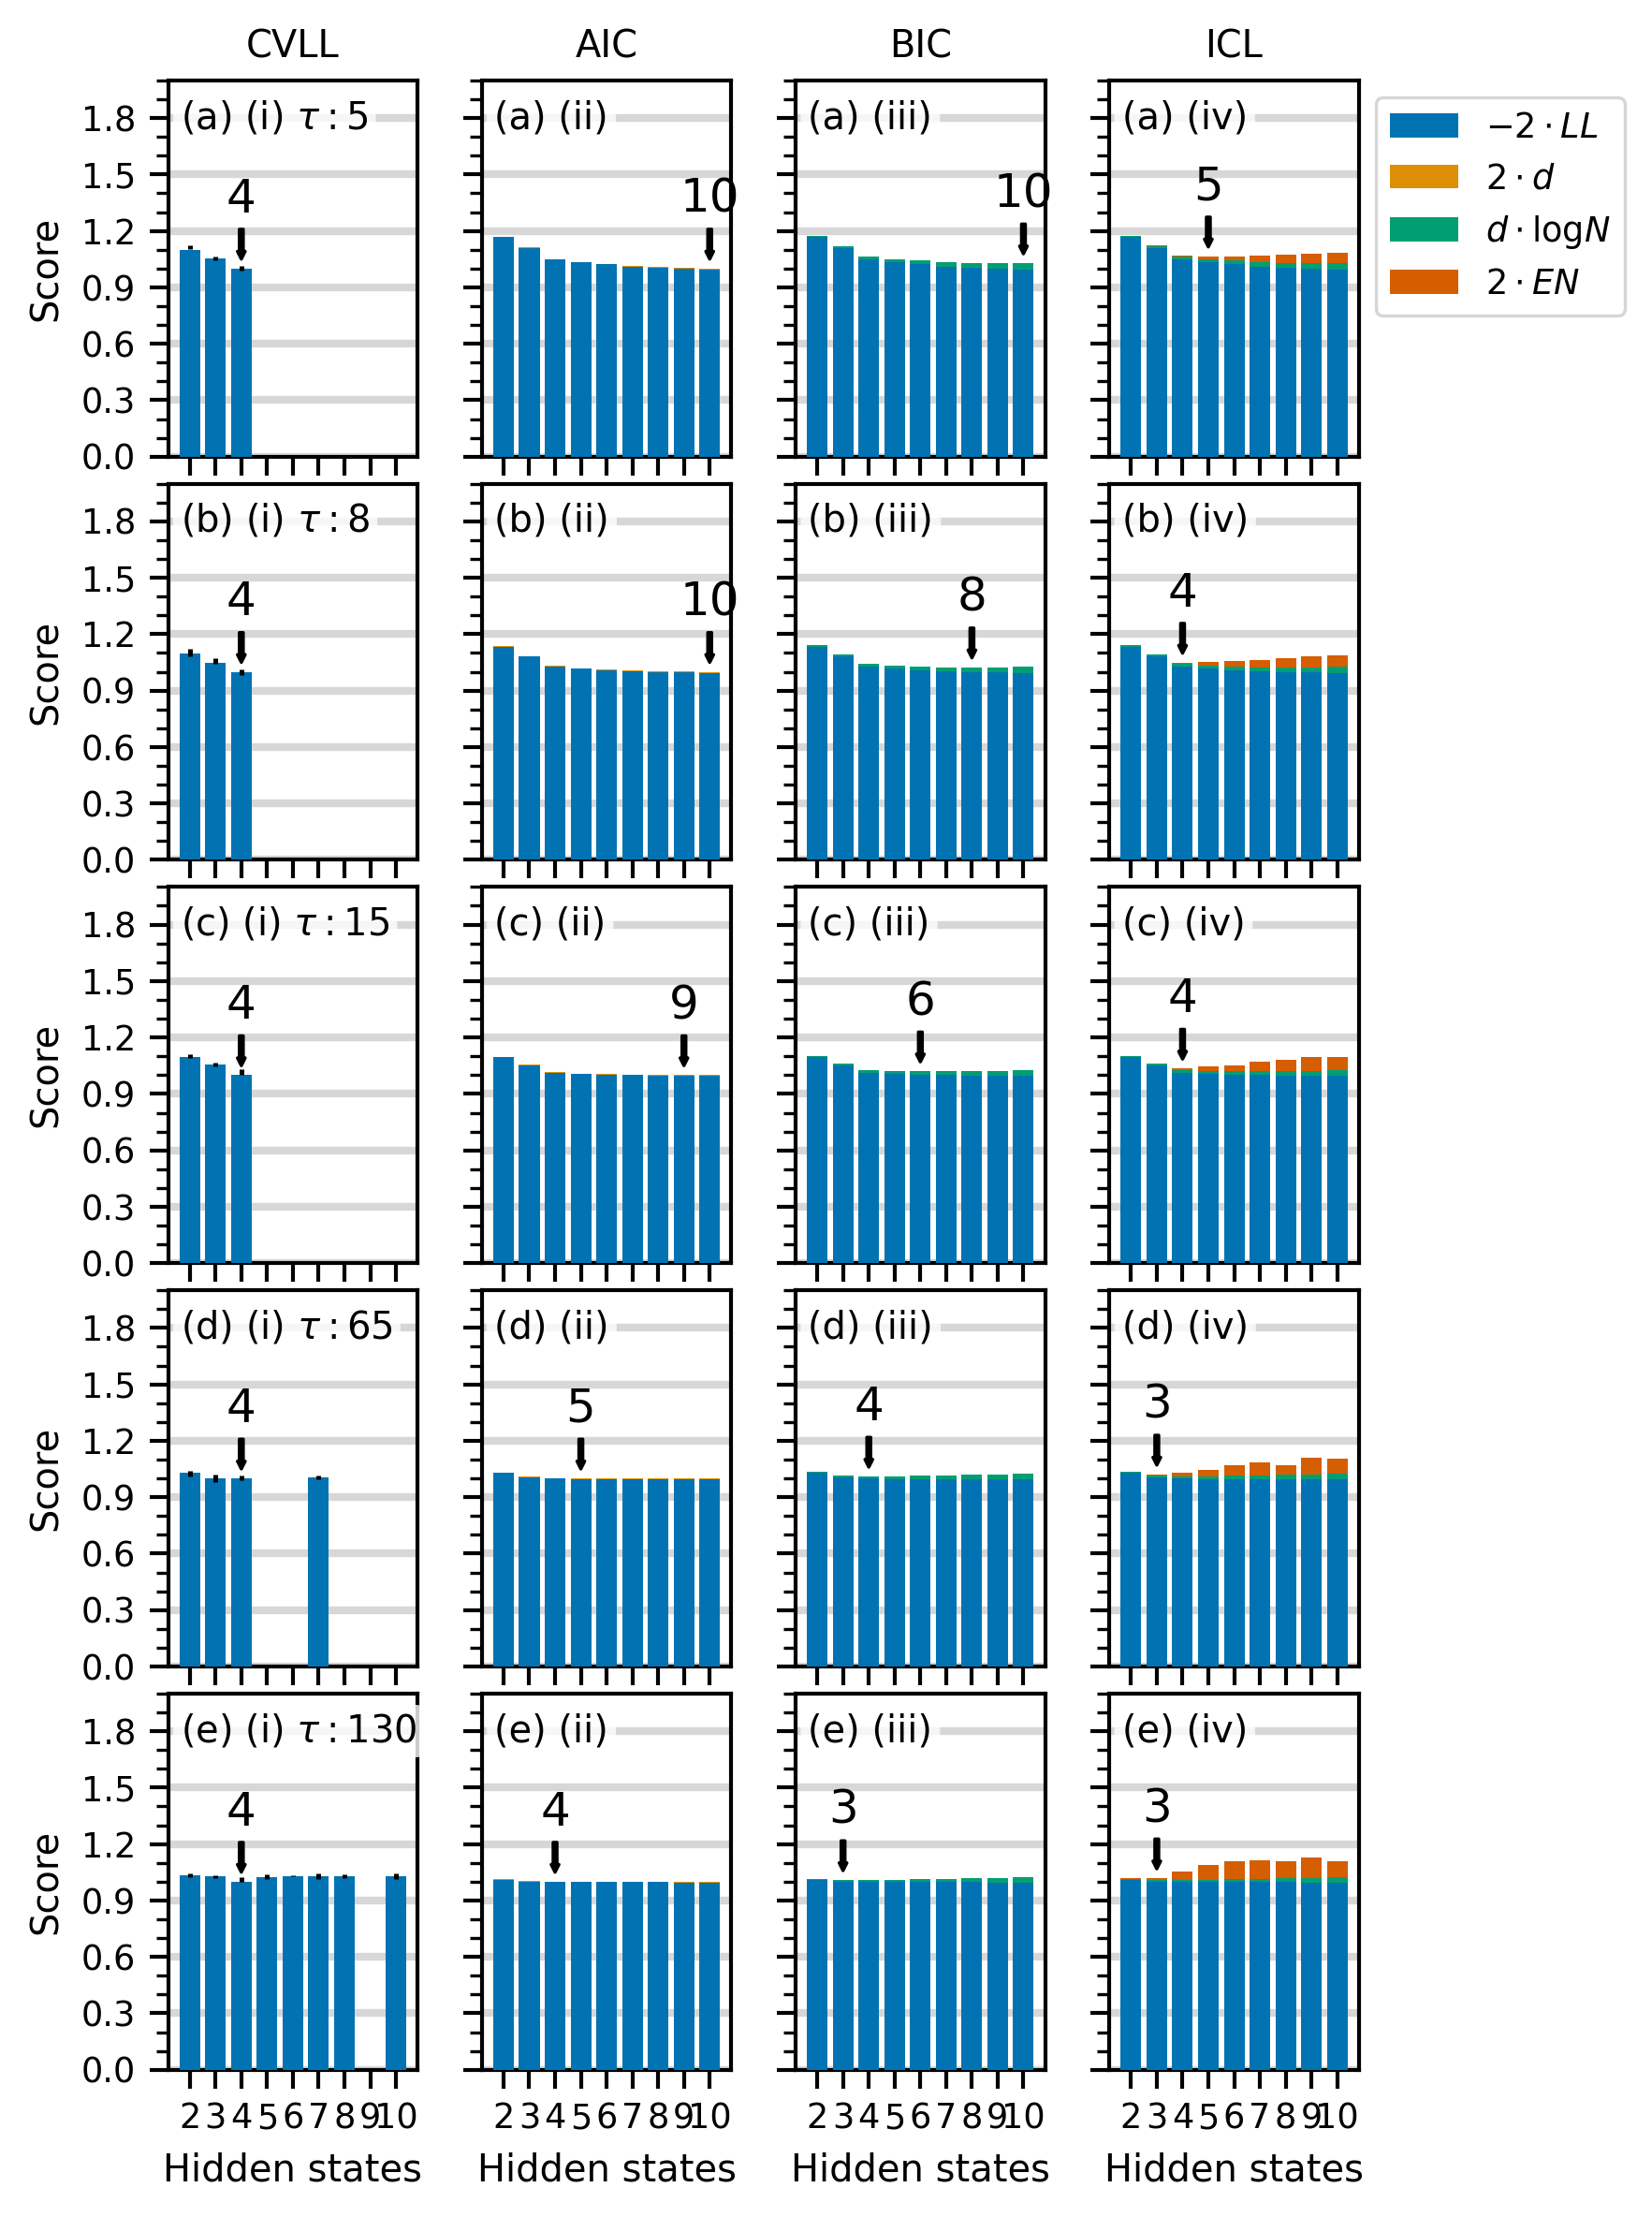
\includegraphics[width=0.75\textwidth]{chapters/hmm_selection/figures/prinz_h_state_selection.png}
    \label{fig:prinz_criteria_results}
\end{figure}

The hidden state selection criteria for HMMs of the Prinz potential are shown in figure \ref{fig:prinz_criteria_results}. Each row, (a) - (e), corresponds to a different value of the Markov lag time $\tau=5, 8, 37, 94, 484$. Each column, (i) - (iv), corresponds to the different model selection criteria, CVLL, AIC, BIC, and ICL. The minimum value of each criteria for each model is highlighted with an arrow indicating the selected number of hidden states. The selection criteria for each model are discussed for each value of $\tau$ below. For each $\tau$ the selected models will be 


% The selected number of hidden states is highlighted with a green disc. No one selection criterion selects the true number of hidden states  for all five values of $\tau$. However, the $\operatorname{ICL}$ criterion, row (h), selects the true number for four models; the $\operatorname{BIC}$, row (f), selects two out of five; the $-\operatorname{CVLL}$ selects one out of five, while the $\operatorname{AIC}$ fails to select any of the true models. All criteria, where they failed to select the true number of states, the selected number of hidden states is over estimated. Also shown in figure \ref{fig:prinz_criteria_results} are the components of the criteria which explain their behaviour. As their 

\subsubsection{Hidden state selection for $\tau=5$}
With $\tau = 5$ the Prinz potential has seven resolvable relaxation processes. The top three form a dominant set, with $t_4 \gg t_5$, whose sign structure partition the $x$ coordinate into four metastable states corresponding to the four potential wells. Can we see four hidden states selected using the various selection criteria and validation tests? 

Points to note: 
\begin{enumerate}
    \item The Chapman-Kolmogorov tests do not differentiate between $g = 2, 3, 4$ states up to $10\tau$ I.e. $T(\tau)^10 = T(10\tau)$ for $g = 2, 3, 4$ hidden states. See figures \ref{fig:prinz_ck_test_5_2} to \ref{fig:prinz_ck_test_5_4}. There's only four states for $\tau < 64$ (the third relaxation process has a lifetime of $64$ time steps. 
    \item There is a cross-validated log likelihood difference between $g = 2 - 4$, see figure \ref{fig:prinz_criteria_results} panel (a)(i) (and for that matter, the non-cross-validated log-likelihood (a)(ii) blue bars) which favours $4$ vs $3,2$. 
    \item However, the likelihood criteria overestimate the number of hidden states. The closest is the ICL with $g=5$. The CK tests for $g=5, 9, 10$ are shown in figures \ref{fig:prinz_ck_test_5_5} - \ref{fig:prinz_ck_test_5_10}. They are re-assuringly rubbish. 
    \item Contra the Noe HMM paper \cite{noeProjectedHiddenMarkov2013a}, increasing the number of hidden states above the `actual' number i.e. $g = 5, 6, 7, 8, 9$, doesn't affect the timescale estimates of the `true' timescales, see figure \ref{fig:prinz_its_tau_5}.
    \item it's puzzling that the likelihood increases for increasing $g$, even the cross-validated value. The likely reason has to do with that the hidden states for $g = 9$ (for instance) overlap a lot. See the lhs panes in figure \ref{fig:prinz_emission_dens_tau_5}.  
    
\end{enumerate}


\begin{figure}
    \centering
    \caption{The emission matrices for HMMs with g = $2, 3, 4, 5 9, 10$ hidden states}
    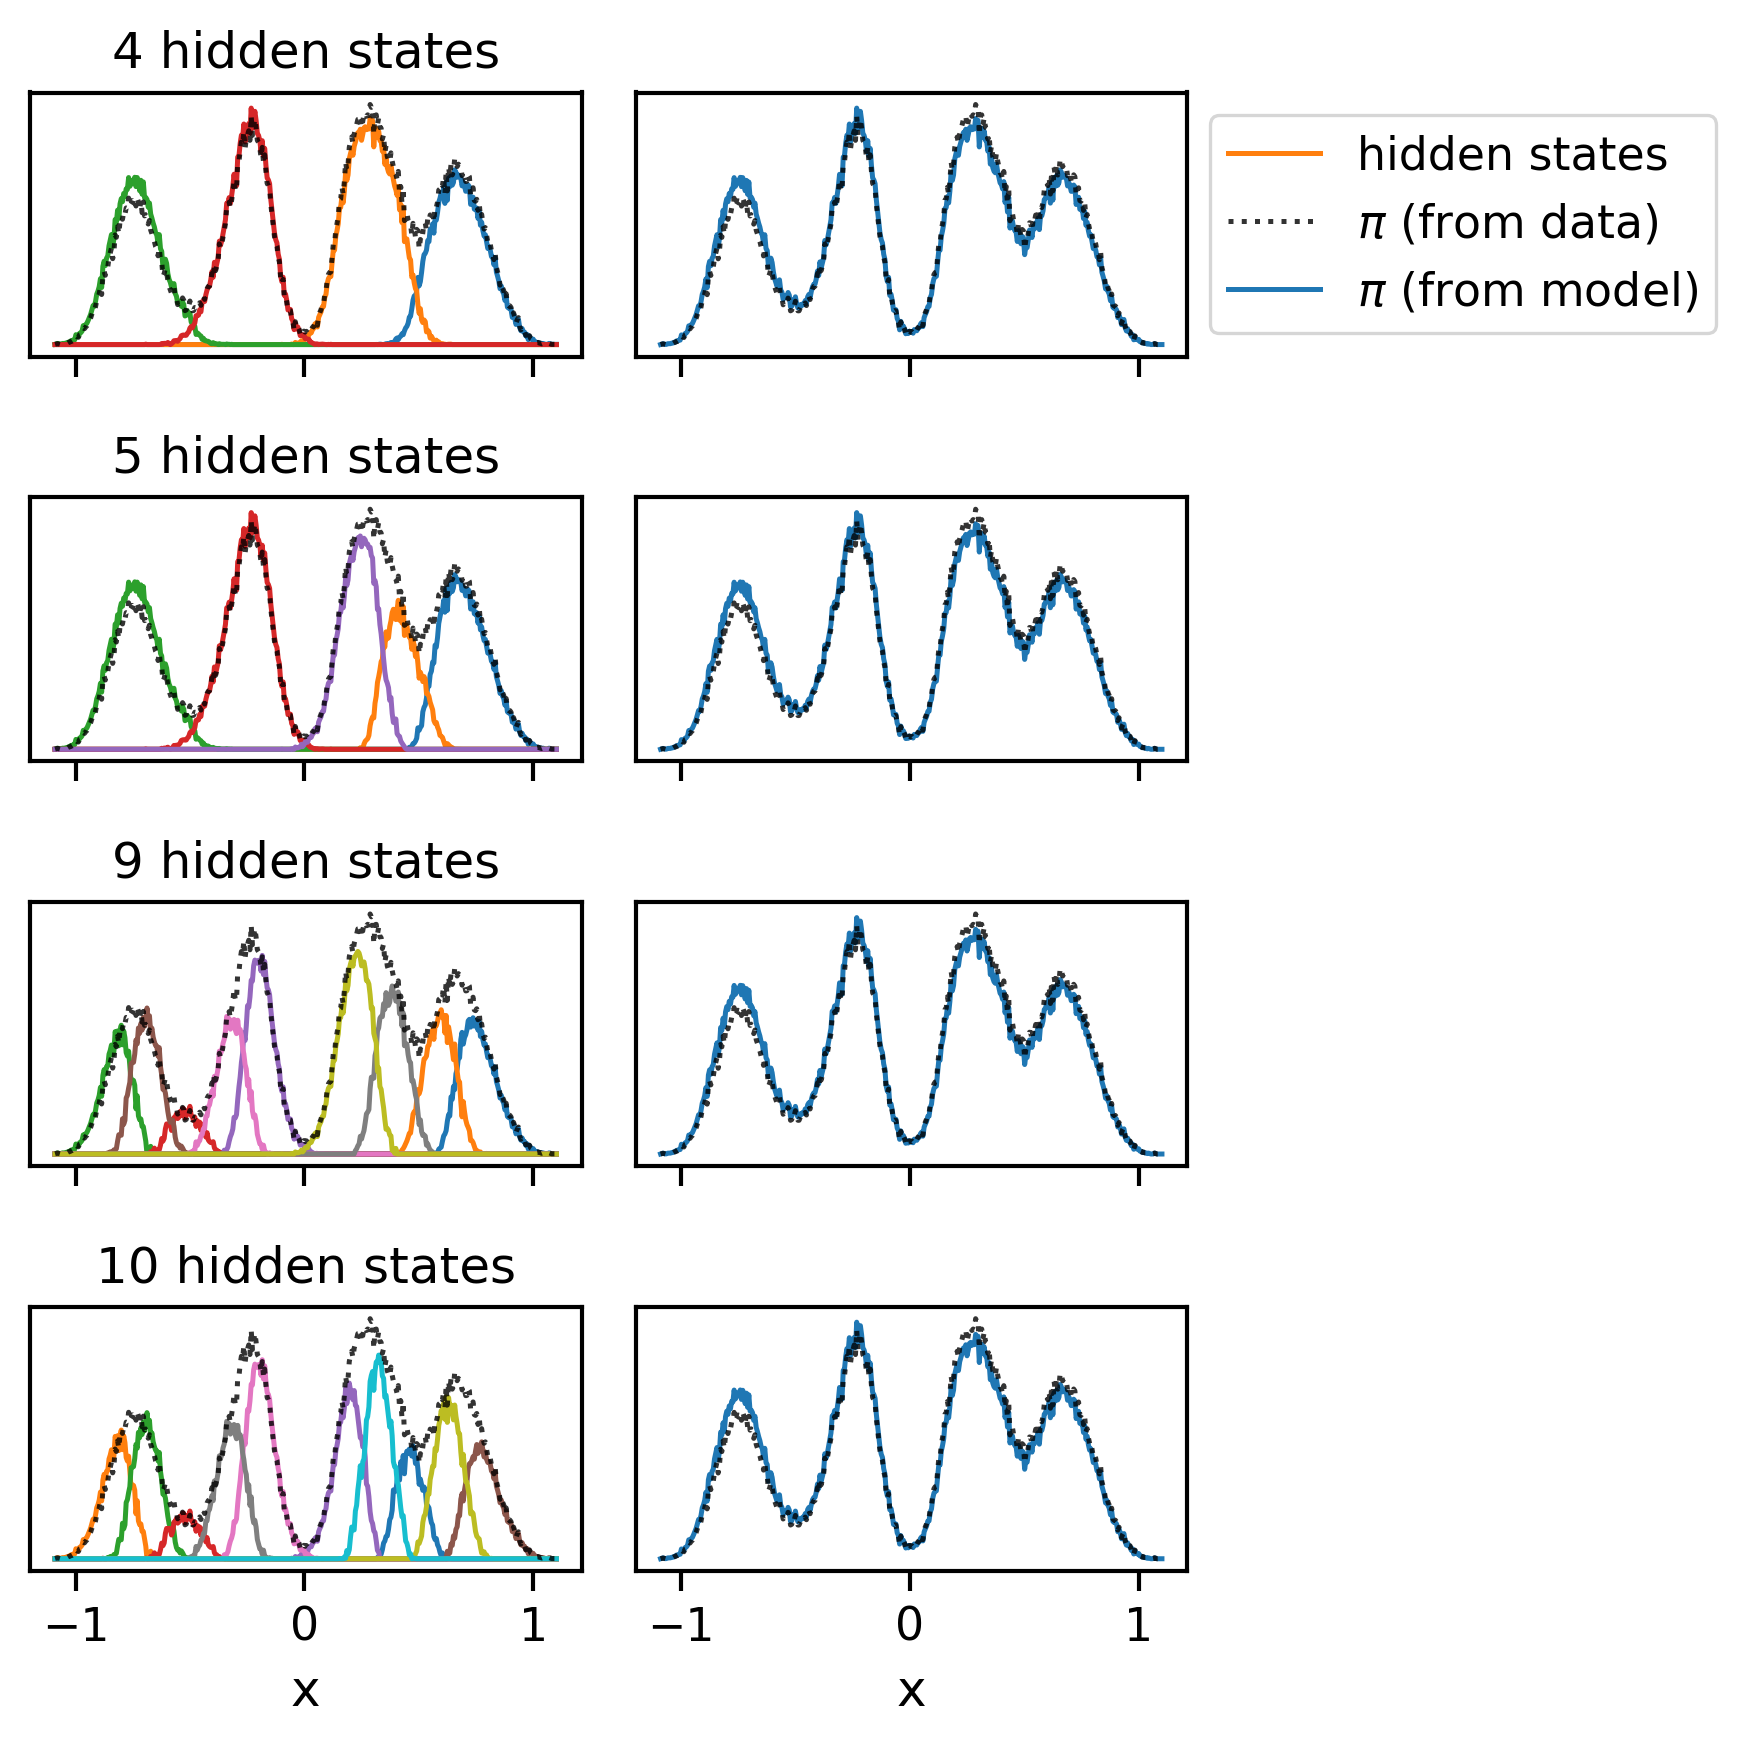
\includegraphics{chapters/hmm_selection/figures/prinz_emitted_densities_tau_5.png}
    \label{fig:prinz_emission_dens_tau_5}
\end{figure}






% A tentative explanation is as follows. The full expression for the observed likelihood for a trajectory of $t$ MD frames is
% \cite{noeProjectedHiddenMarkov2013a}: 

% \begin{equation}
% \mathbb{P}\left(\left\{s_{t}\right\} \mid \tilde{\mathbf{T}}, \mathbf{E}\right)=\sum_{\text {hidden paths }} \tilde{\pi}_{h_{0}} \mathbf{E}_{s_{0} h_{0}} \prod_{t=1}^{t_{\max }} \tilde{T}_{h_{t-1} h_{t}} \mathbf{E}_{s_{t} h_{t}},
% \end{equation}

% with initial distribution $\tilde{\pi}_{h_{0}}$ is approximated by the stationary distribution, $\tilde{\pi}$.  For each hidden path, i.e. the sequence of hidden states for each frame of the MD trajectory, the likelihood is comprised of the $t$ products of the probability of transitioning into a hidden state $h_j$, and the conditional probability of observing a state $s_i$ given the hidden state. 
% [More explanation]




\subsection{AADH}

\section{Conclusions}

\section{Appendix}


% \begin{figure}
%     \centering
%     \begin{minipage}{0.4\textwidth}
%         \centering 
%          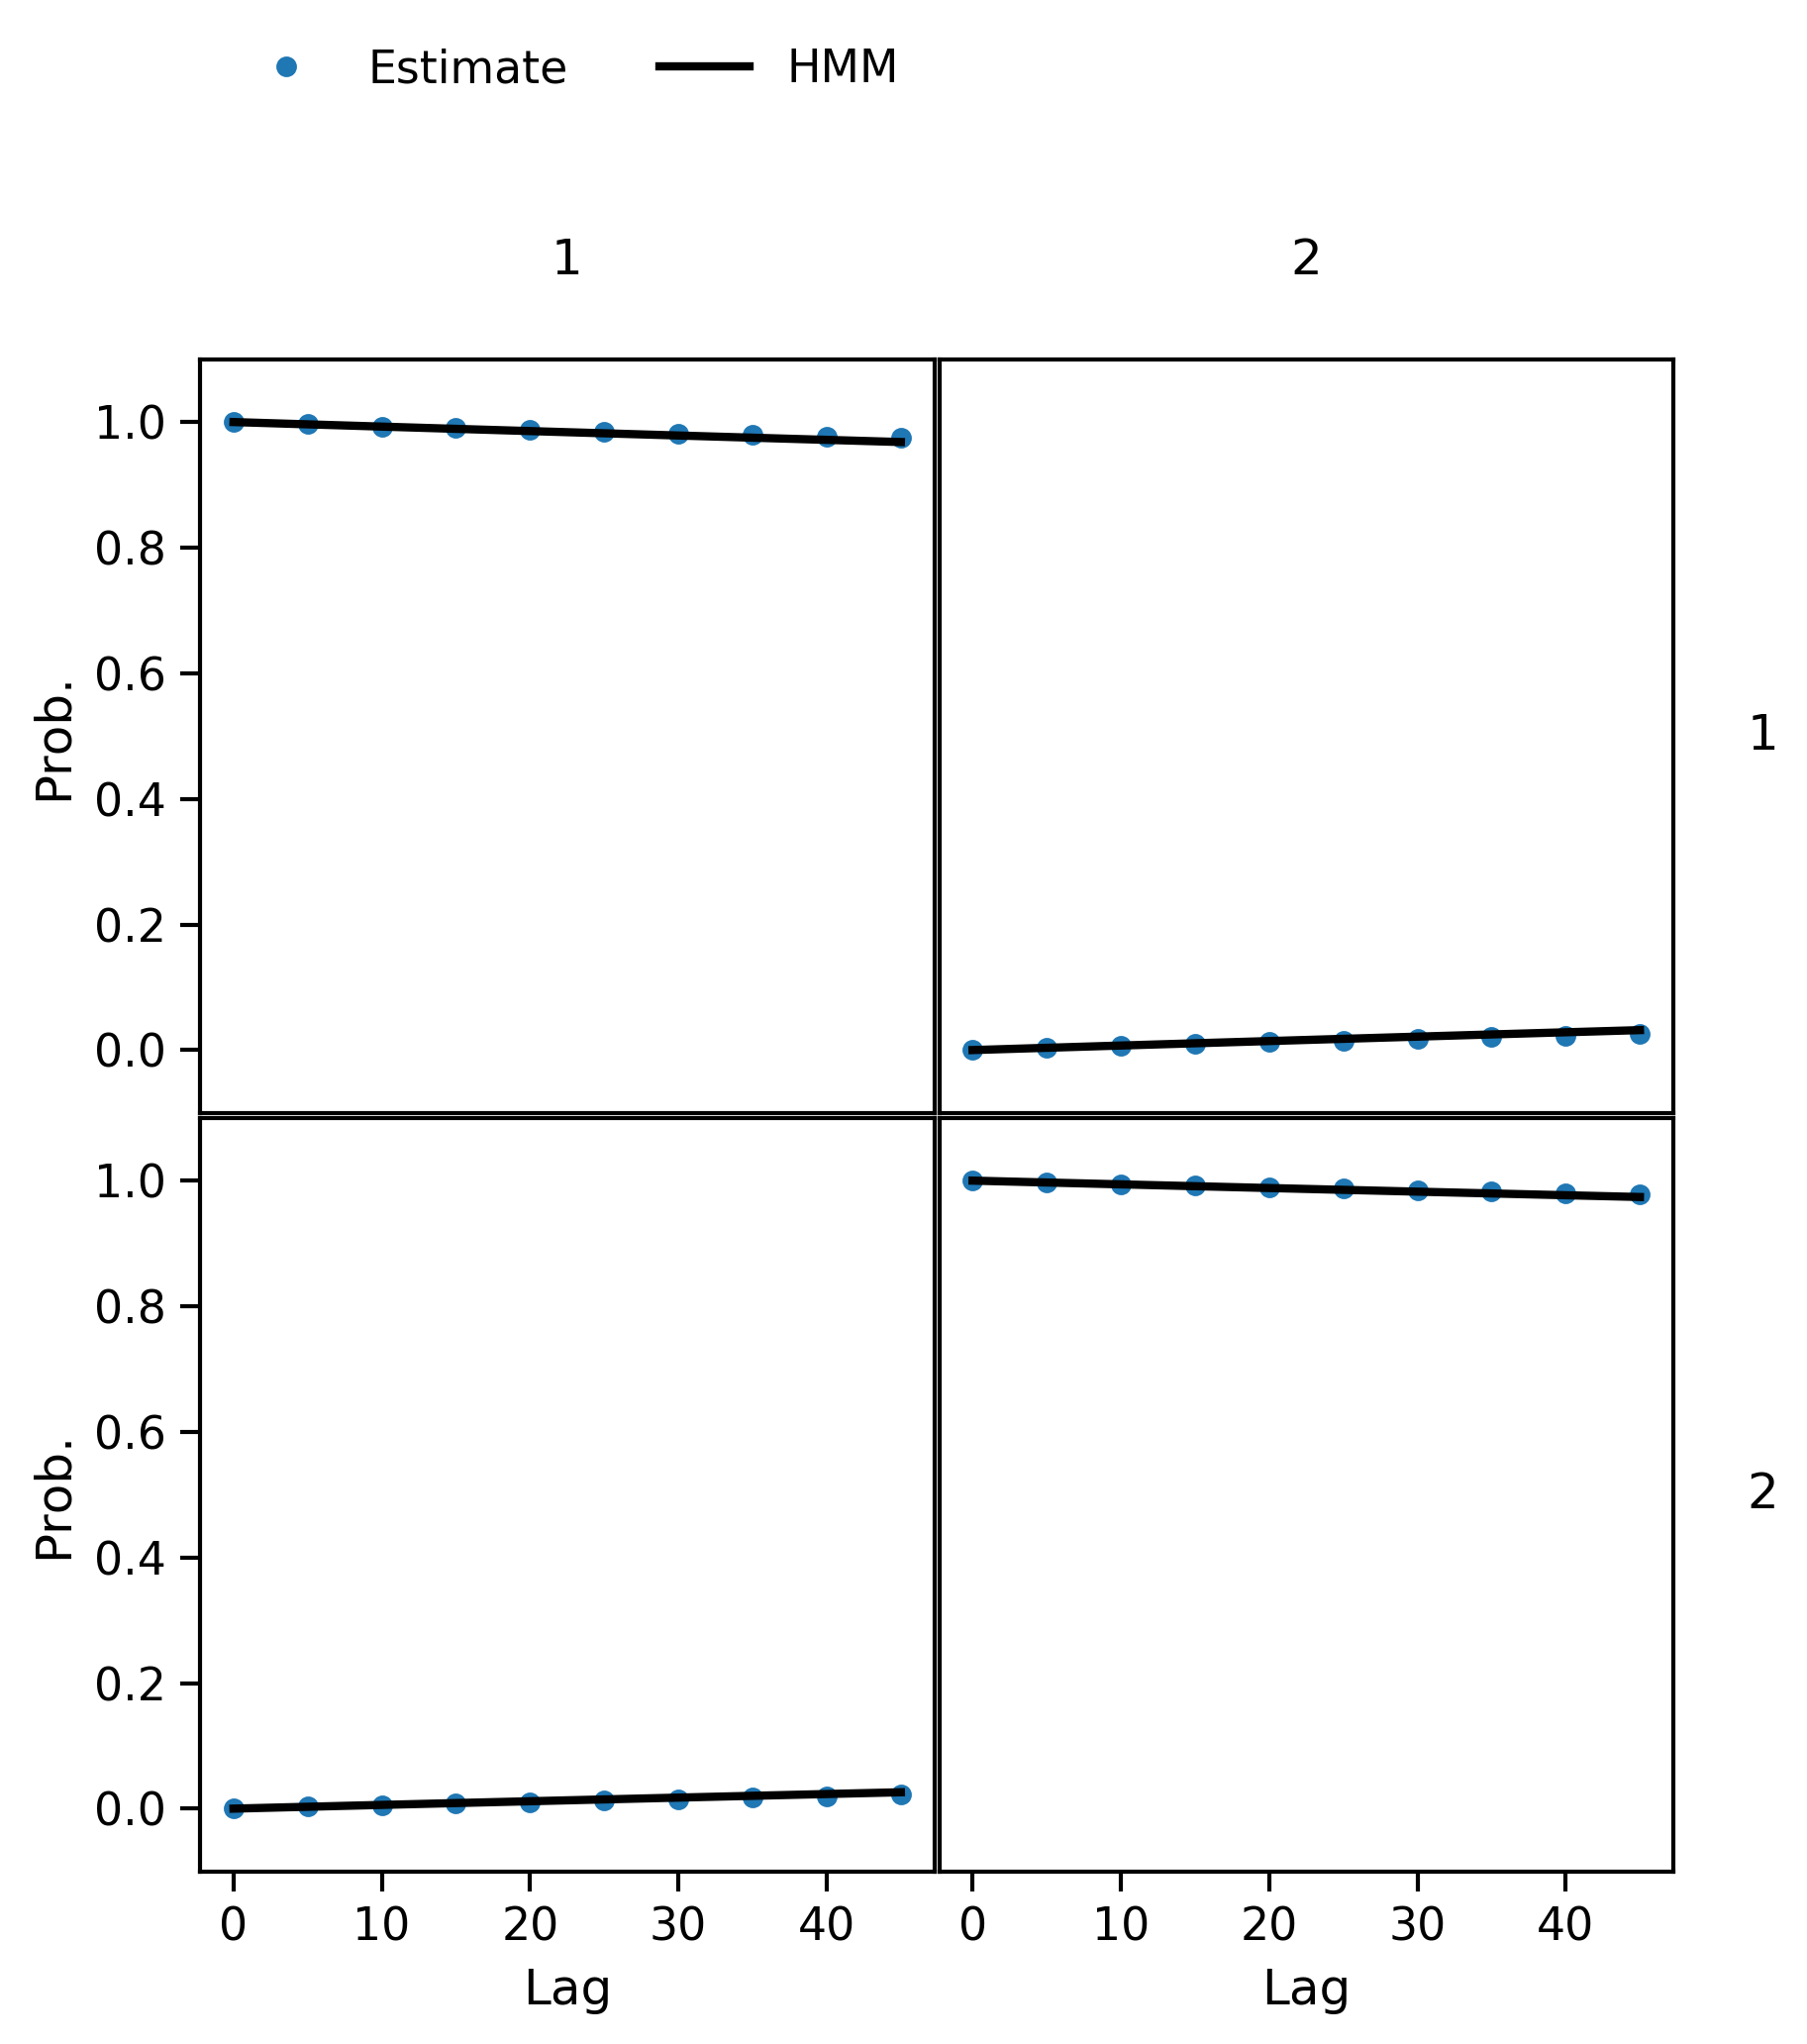
\includegraphics[width=0.8\linewidth]{chapters/hmm_selection/figures/ck_test_5_2.png}
%         \caption{CK test for Prinz Potential with $\tau=5$ and $g=2$} \label{fig:prinz_ck_test_5_2}
%     \end{minipage}
%     \hfill
%     \begin{minipage}{0.4\textwidth}
%         \centering
%          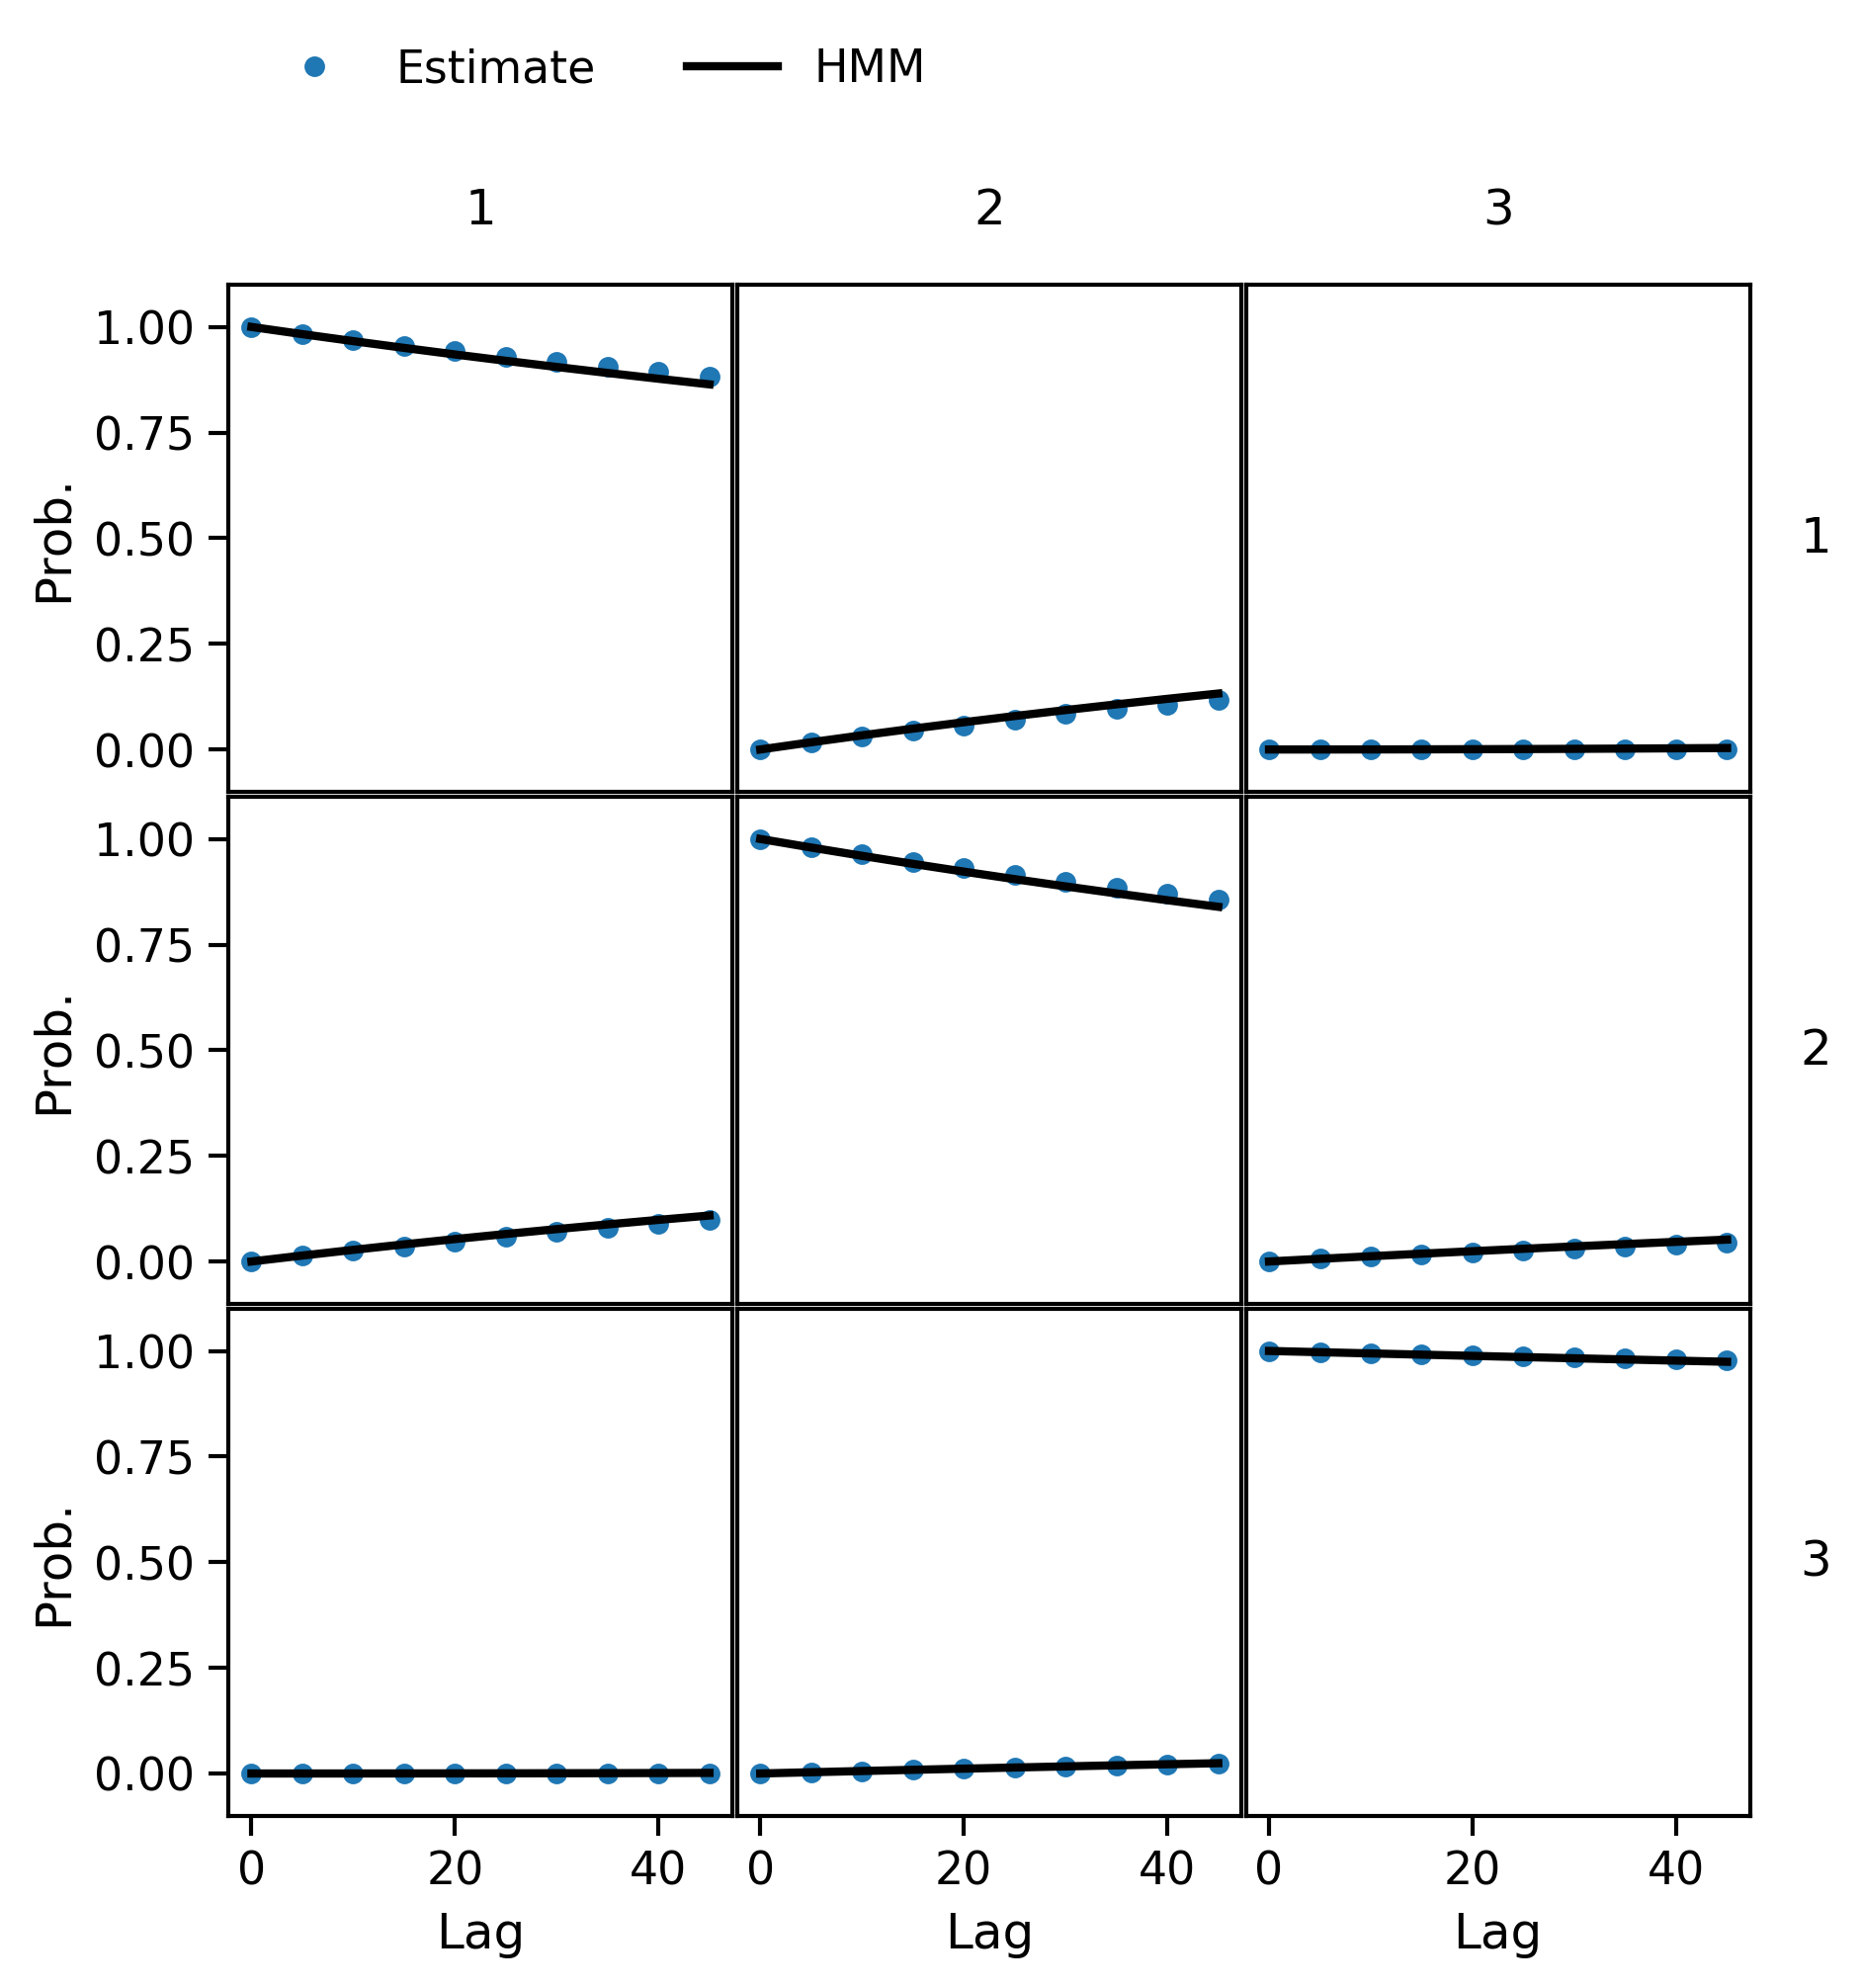
\includegraphics[width=0.8\linewidth]{chapters/hmm_selection/figures/ck_test_5_3.png}
%         \caption{CK test for Prinz Potential with $\tau=5$ and $g=3$} \label{fig:prinz_ck_test_5_3}
%     \end{minipage}
% \end{figure}



% \begin{figure}[p]
%     \centering
%     \mycaption{CK tests for Prinz Potential with $\tau = 5$ and $g = 2, 3$}
%     \subtop[$g = 2$]{
%         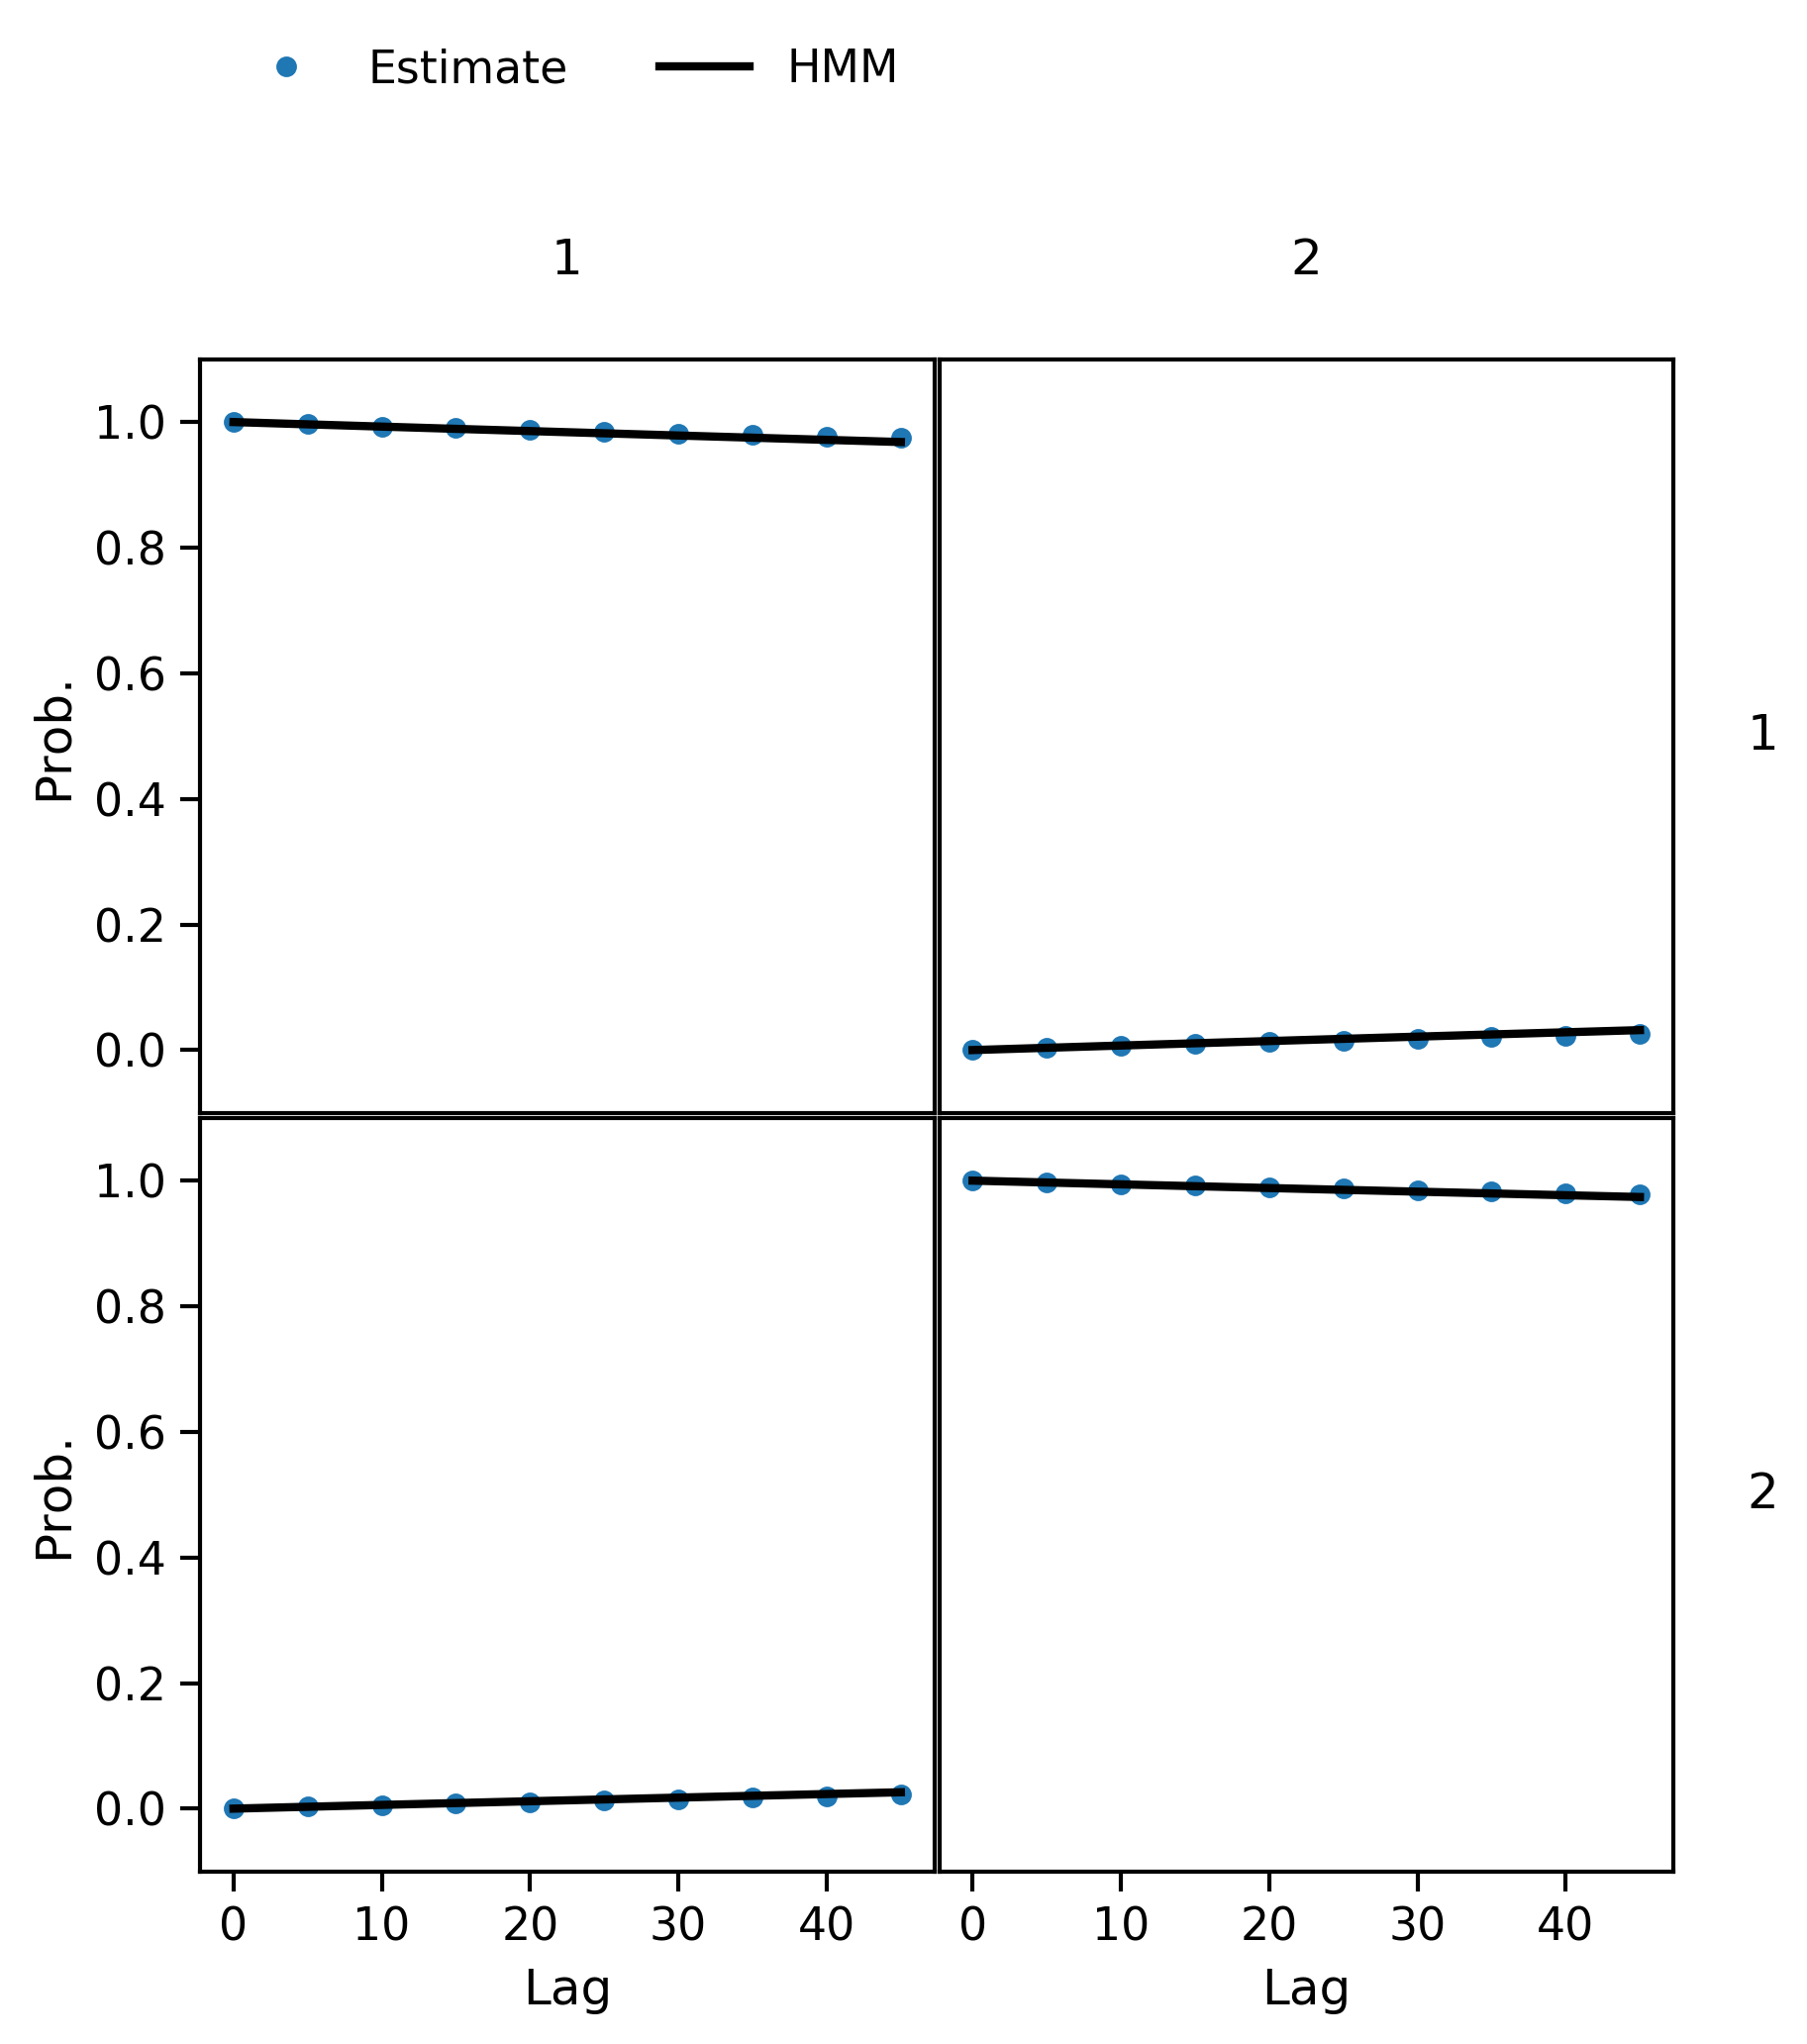
\includegraphics[width=0.4\textwidth]{chapters/hmm_selection/figures/ck_test_5_2.png}}
    
%     \subtop[$g = 3$]{
%         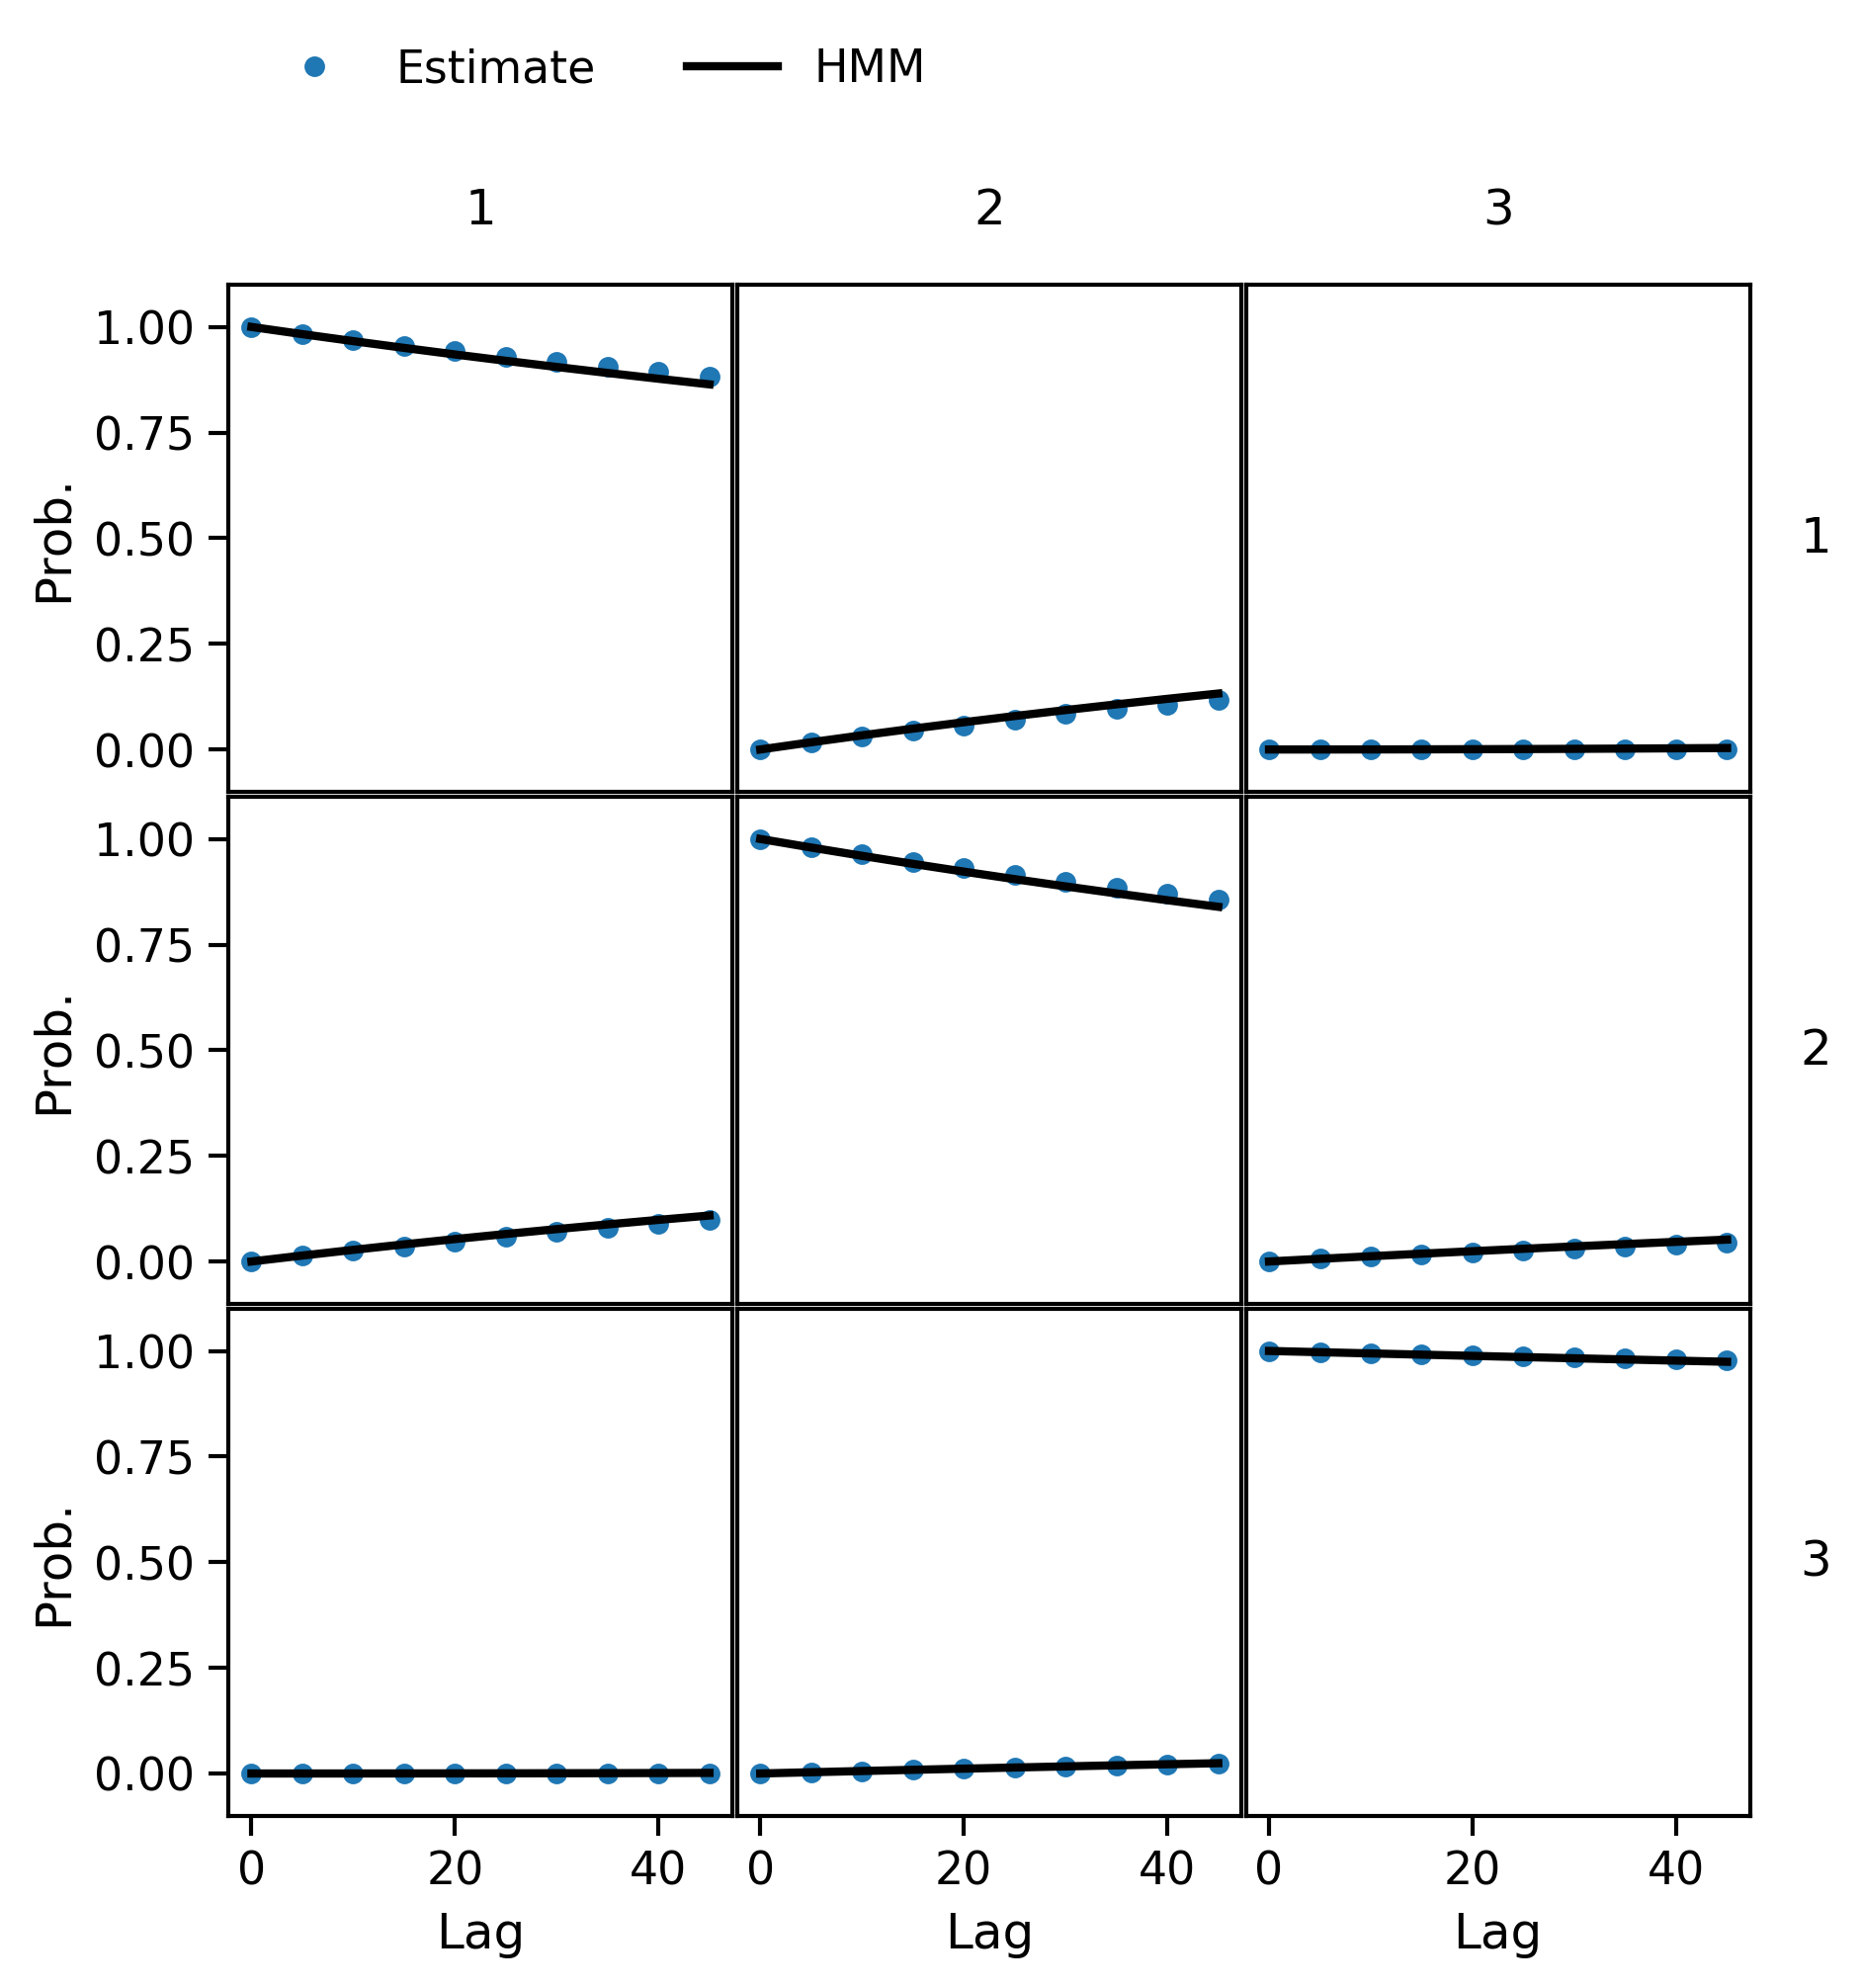
\includegraphics[width=0.4\textwidth]{chapters/hmm_selection/figures/ck_test_5_3.png}}
% \end{figure}

\begin{figure}
    \centering
    \mycaption{CK test for Prinz Potential with $\tau=5$ and $g=2$}
    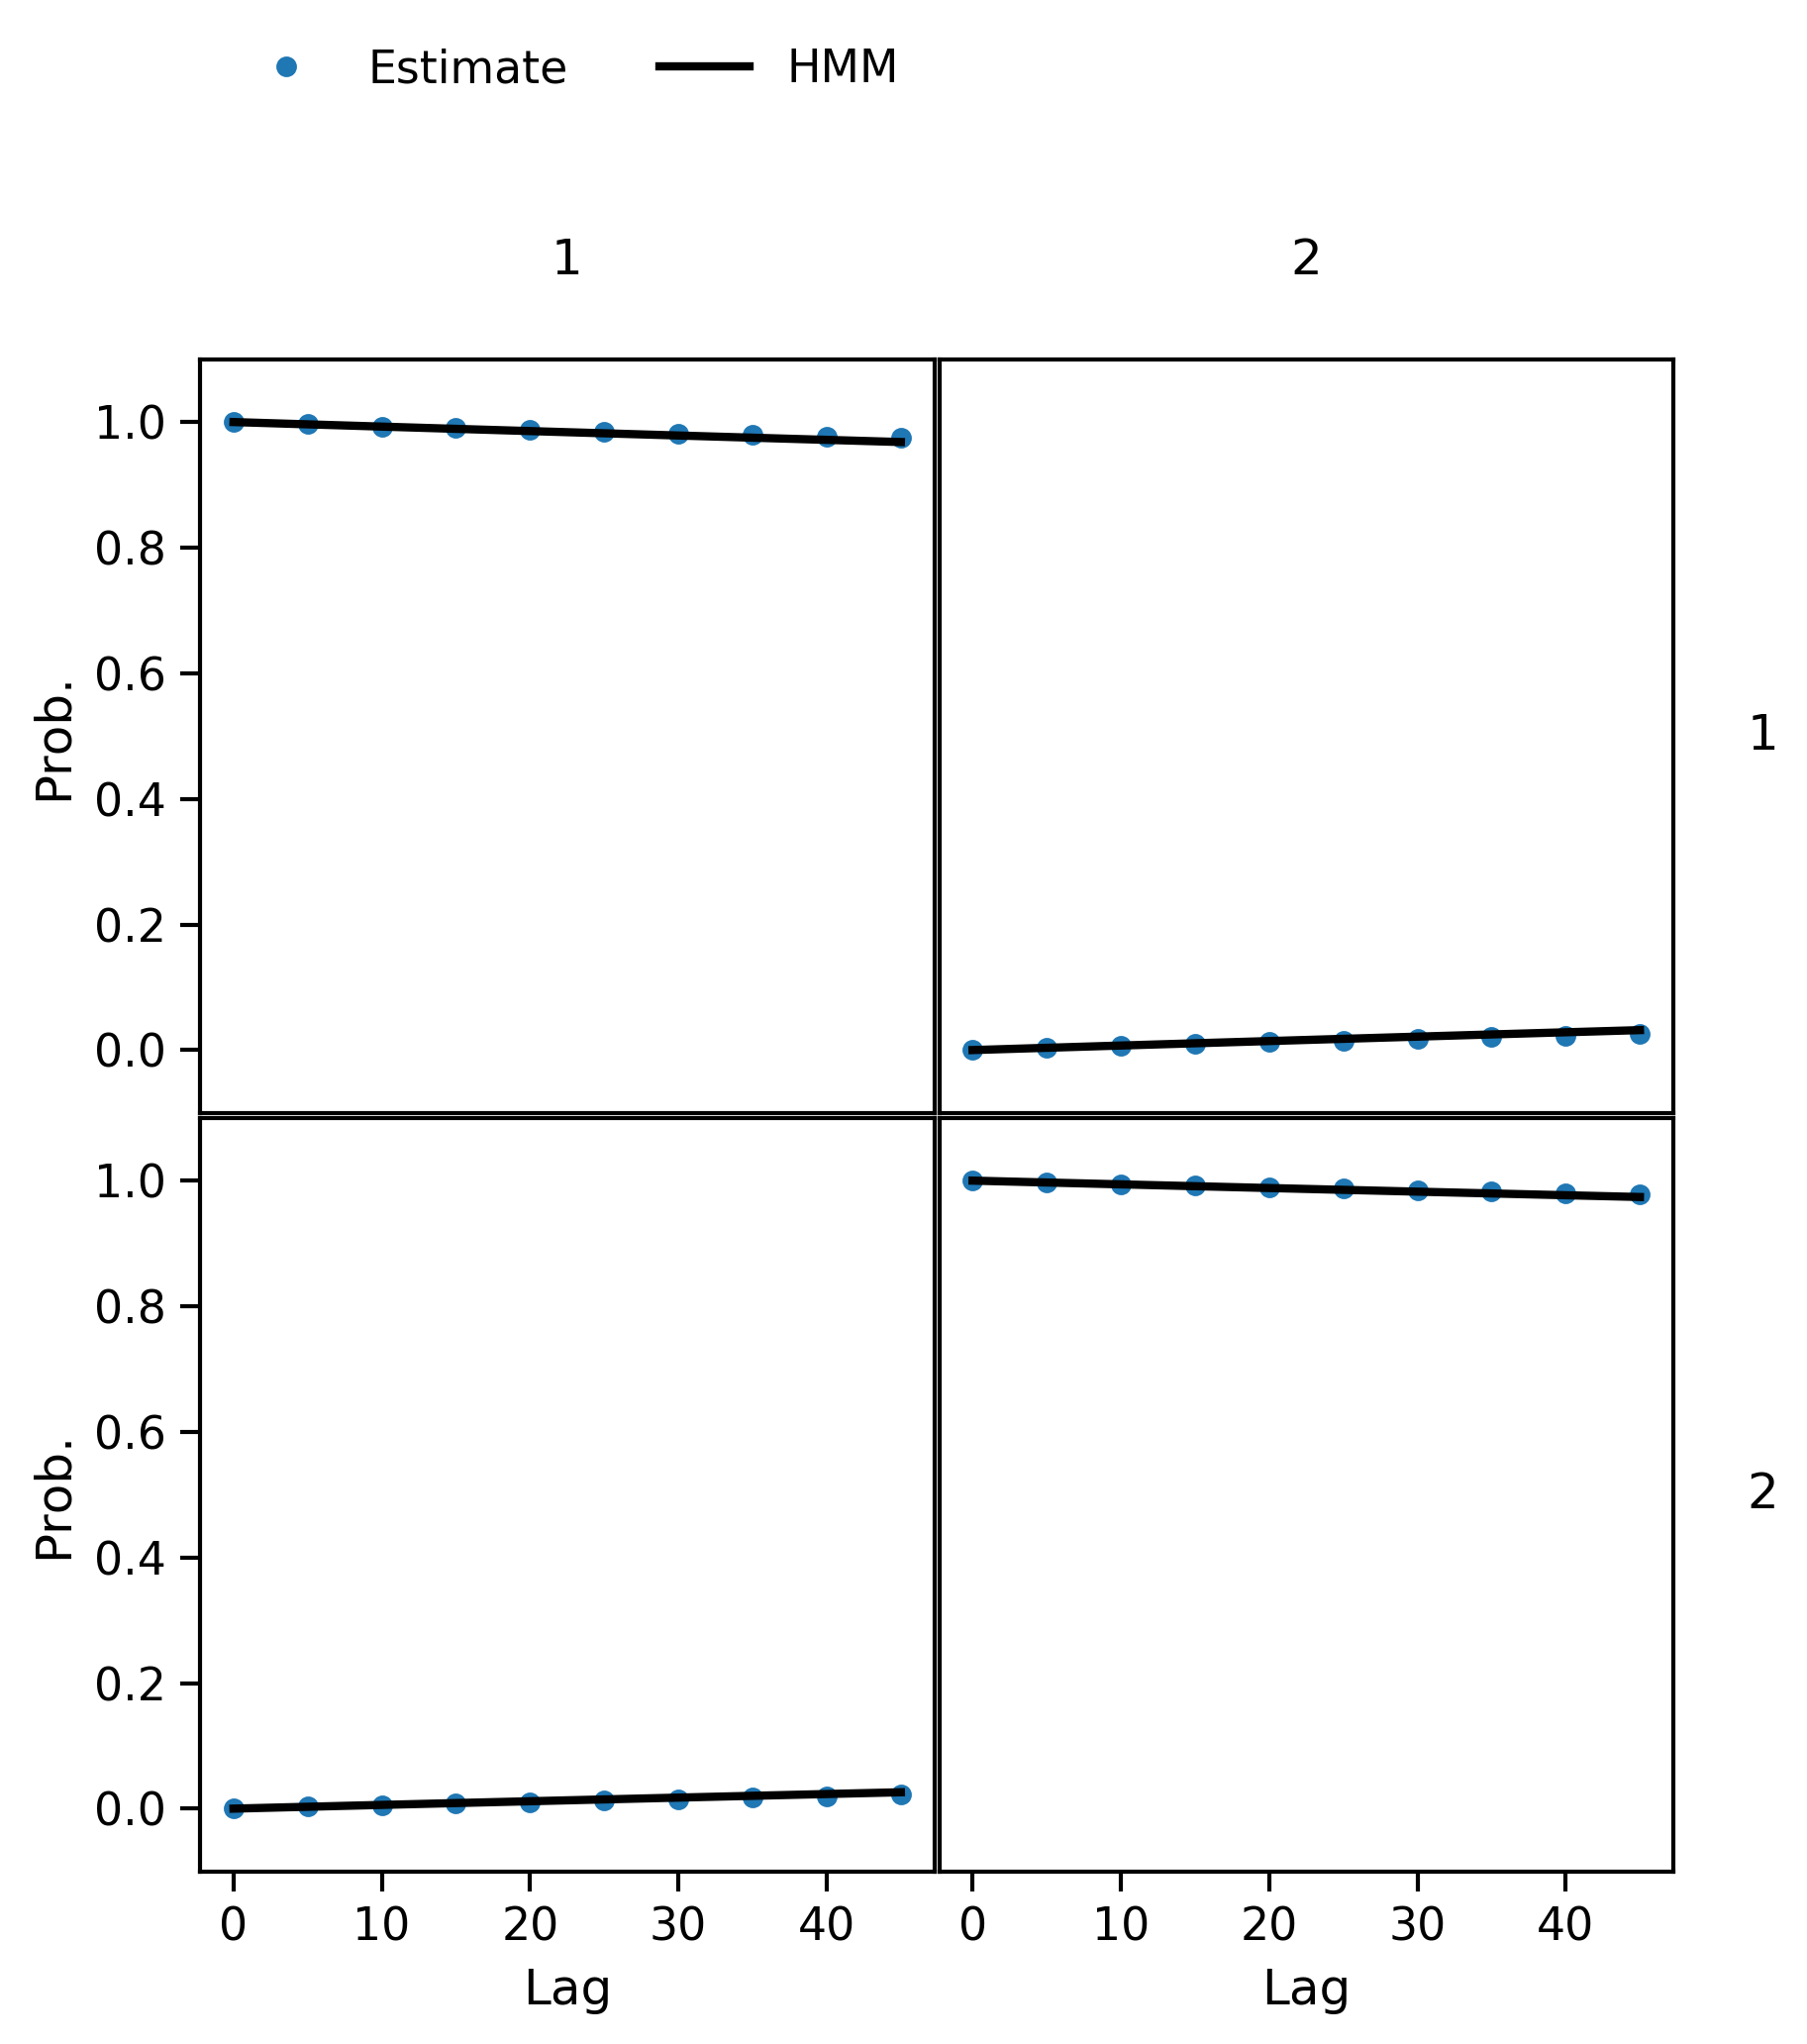
\includegraphics{chapters/hmm_selection/figures/ck_test_5_2.png}
    
    \label{fig:prinz_ck_test_5_2}
\end{figure}


\begin{figure}
    \centering
    \mycaption{CK test for Prinz Potential with $\tau=5$ and $g=3$}
    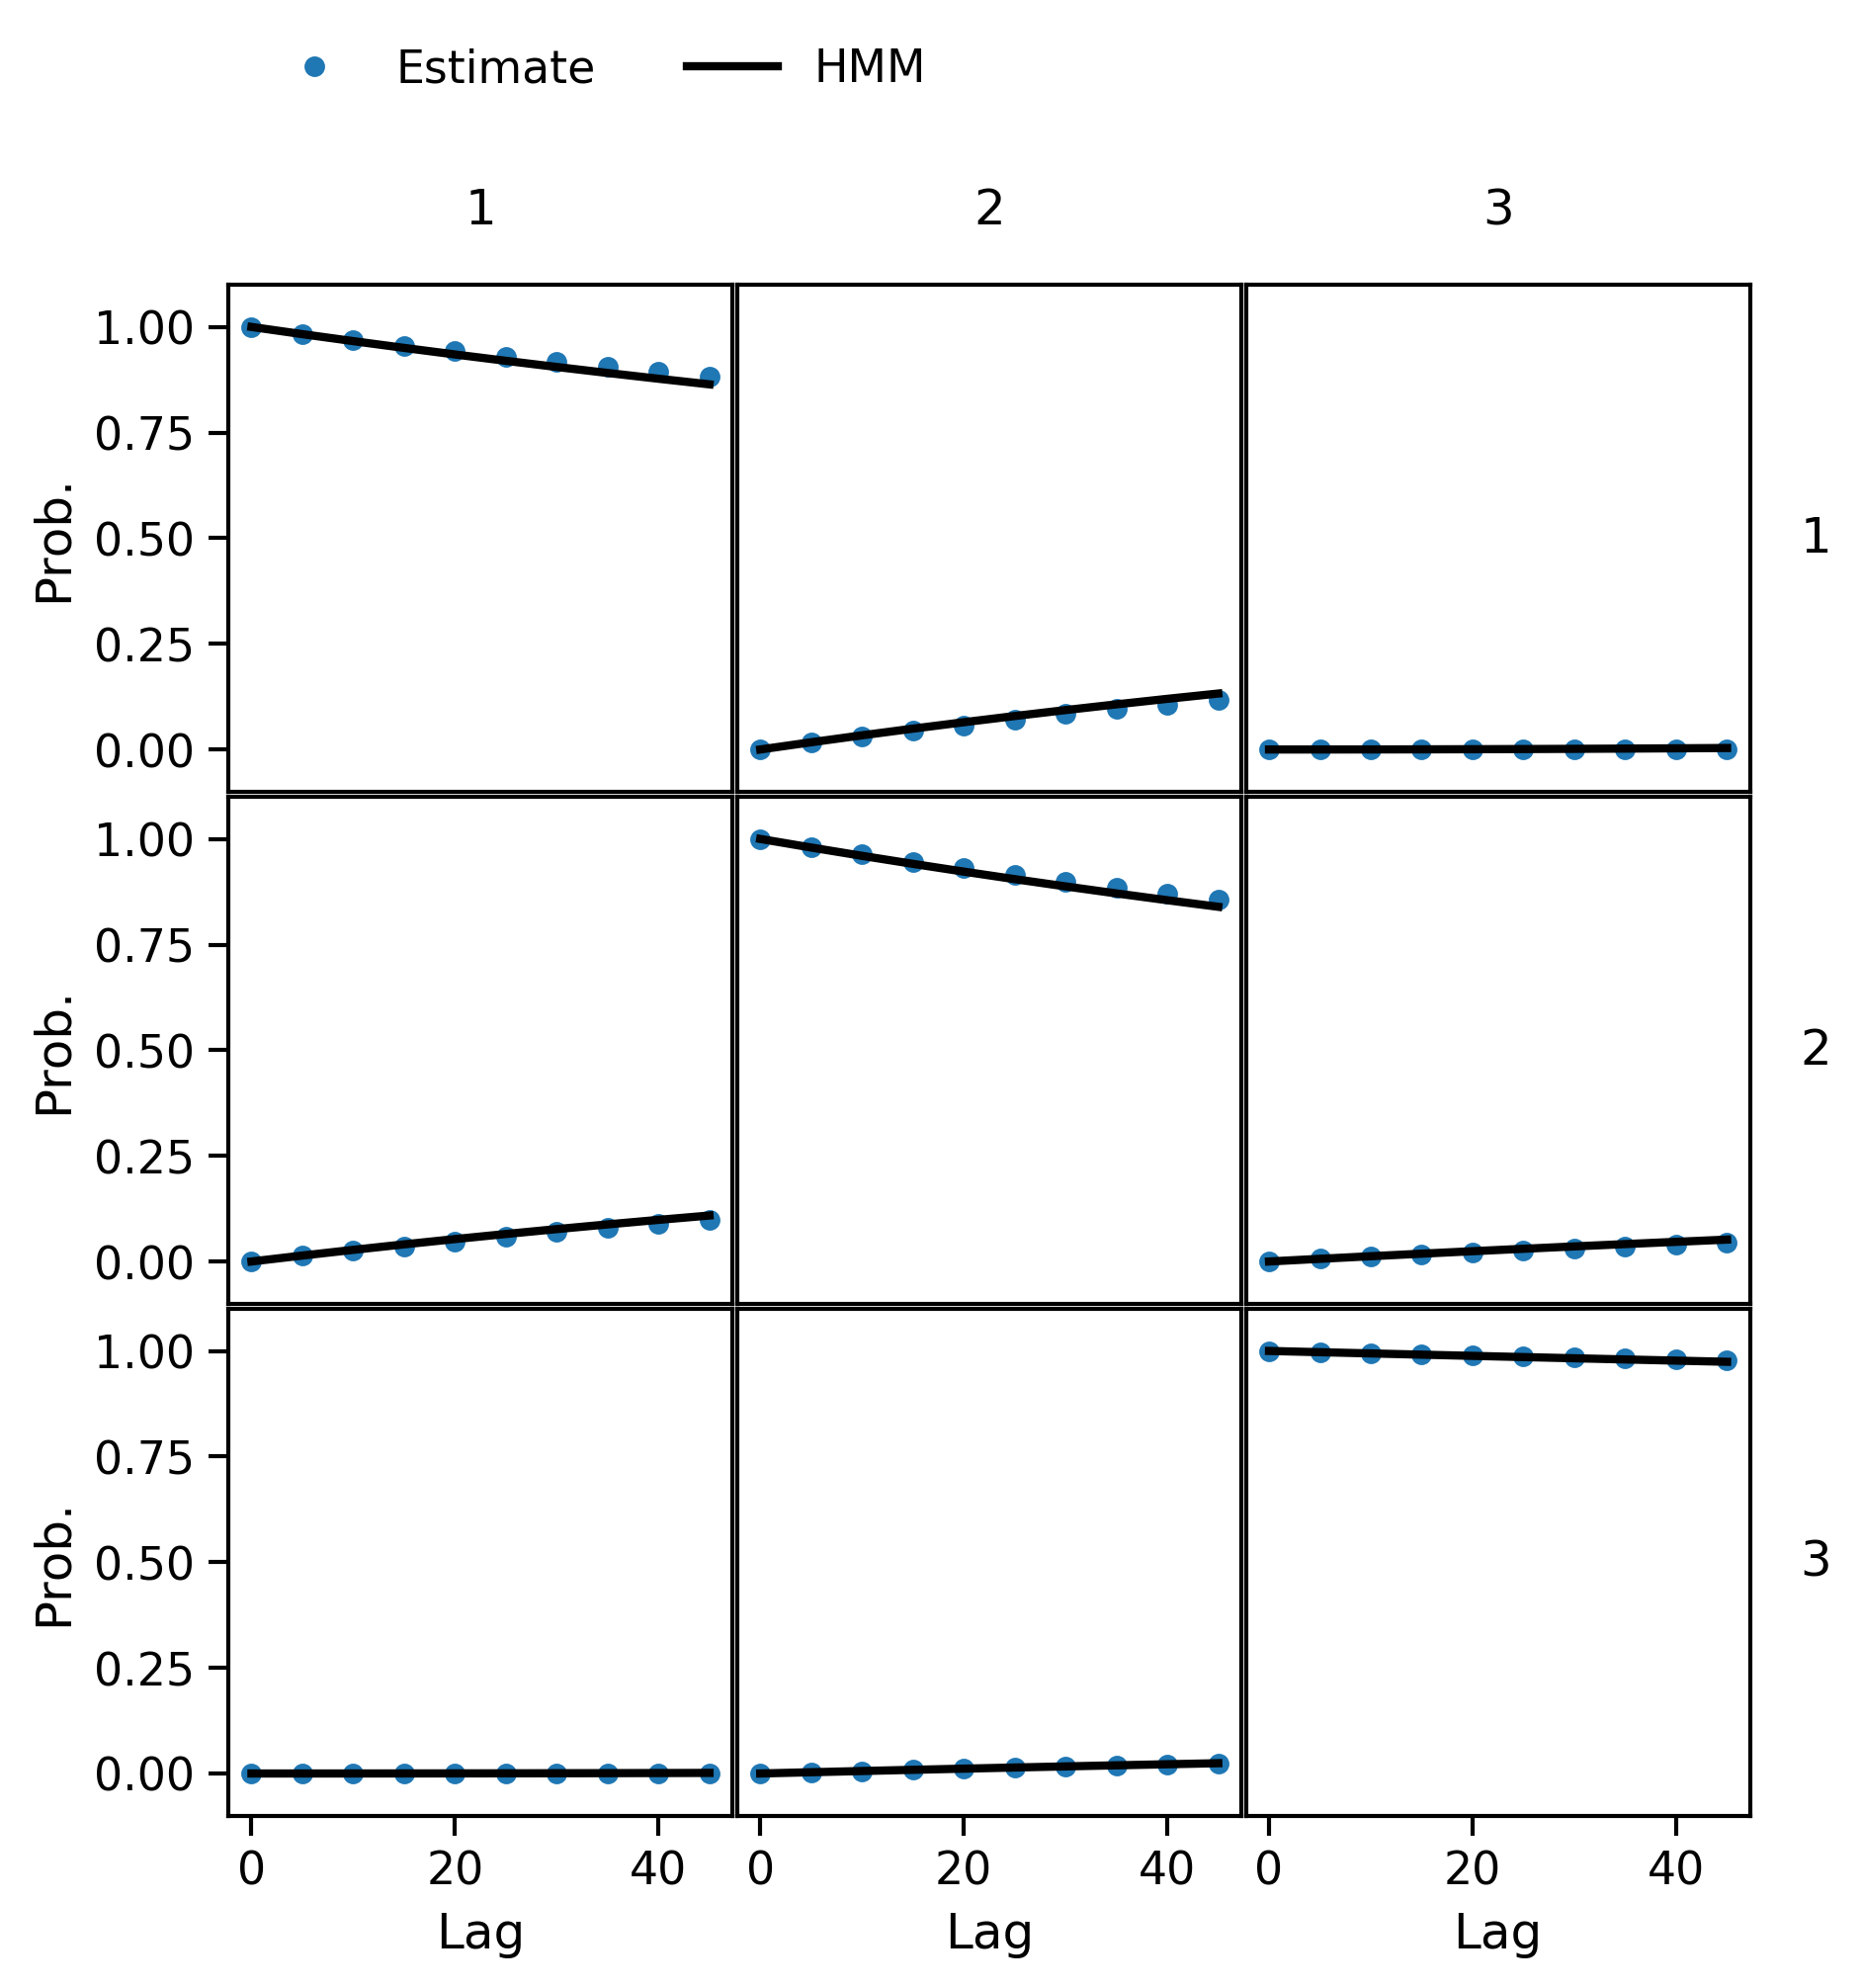
\includegraphics{chapters/hmm_selection/figures/ck_test_5_3.png}
    
    \label{fig:prinz_ck_test_5_3}
\end{figure}

\begin{figure}
    \centering
    \mycaption{CK test for Prinz Potential with $\tau=5$ and $g=4$}
    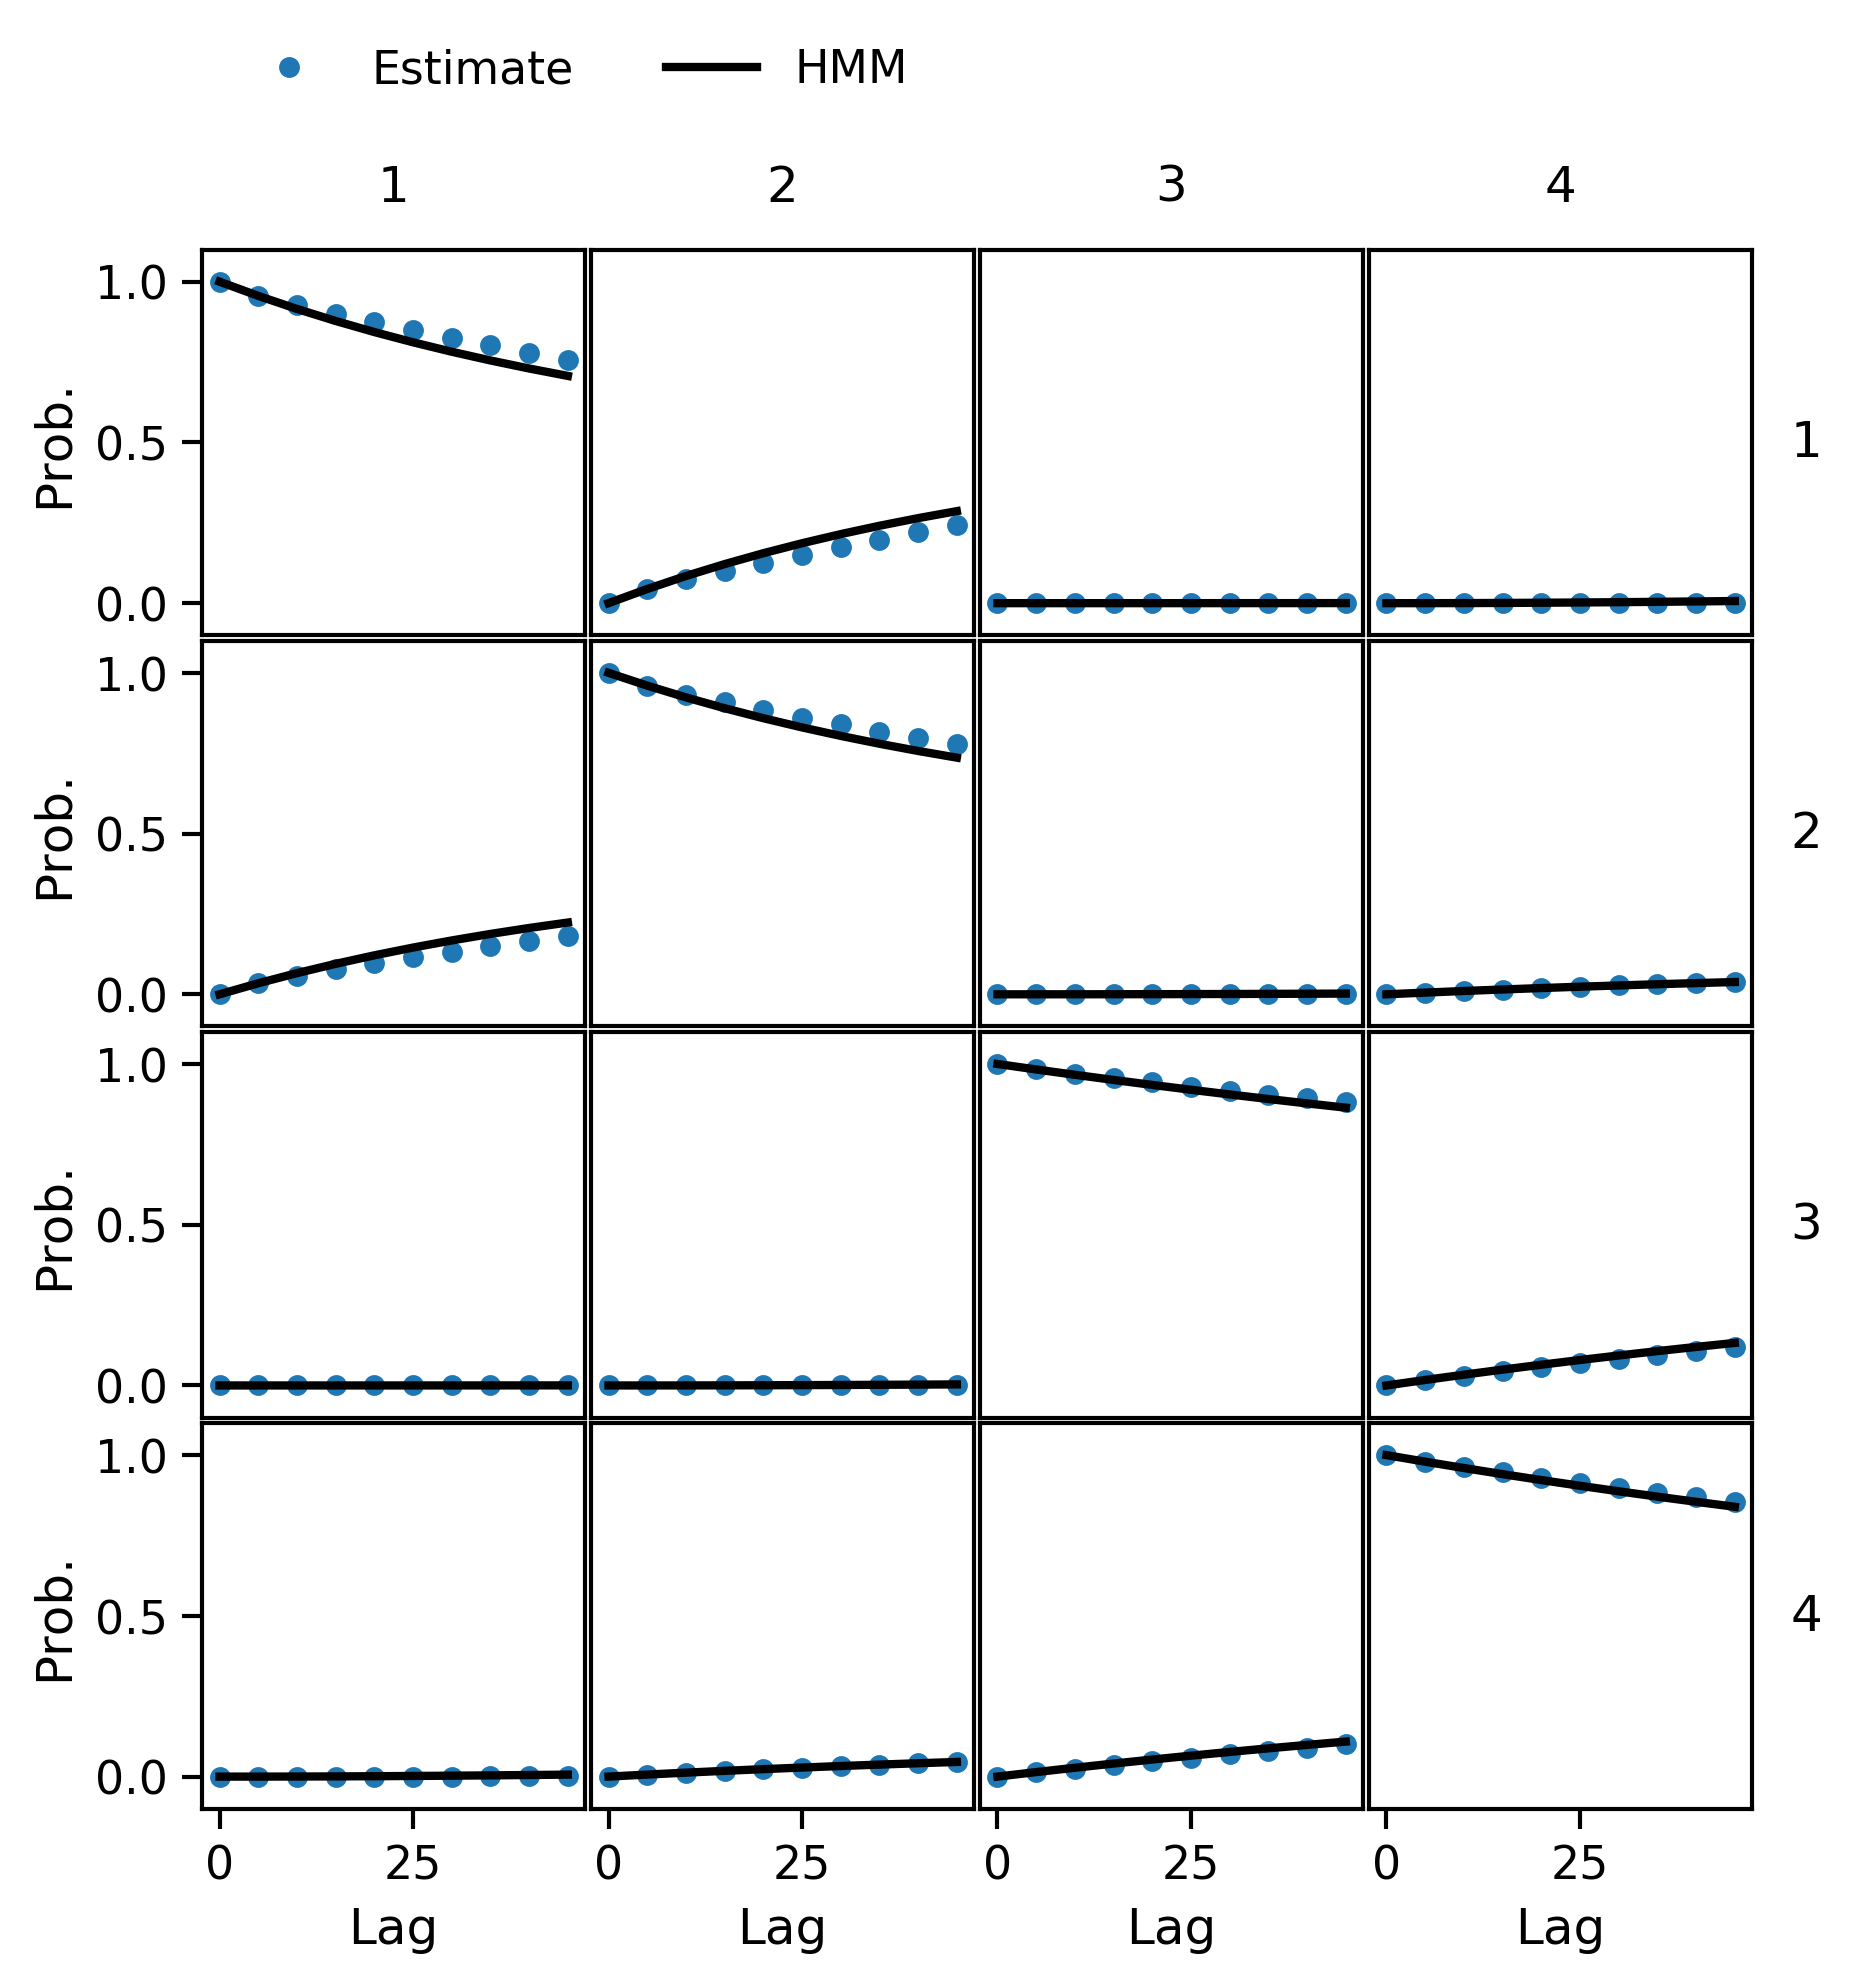
\includegraphics{chapters/hmm_selection/figures/ck_test_5_4.png}
    
    \label{fig:prinz_ck_test_5_4}
\end{figure}

\begin{figure}
    \centering
    \mycaption{CK test for Prinz Potential with $\tau=5$ and $g=5$}
    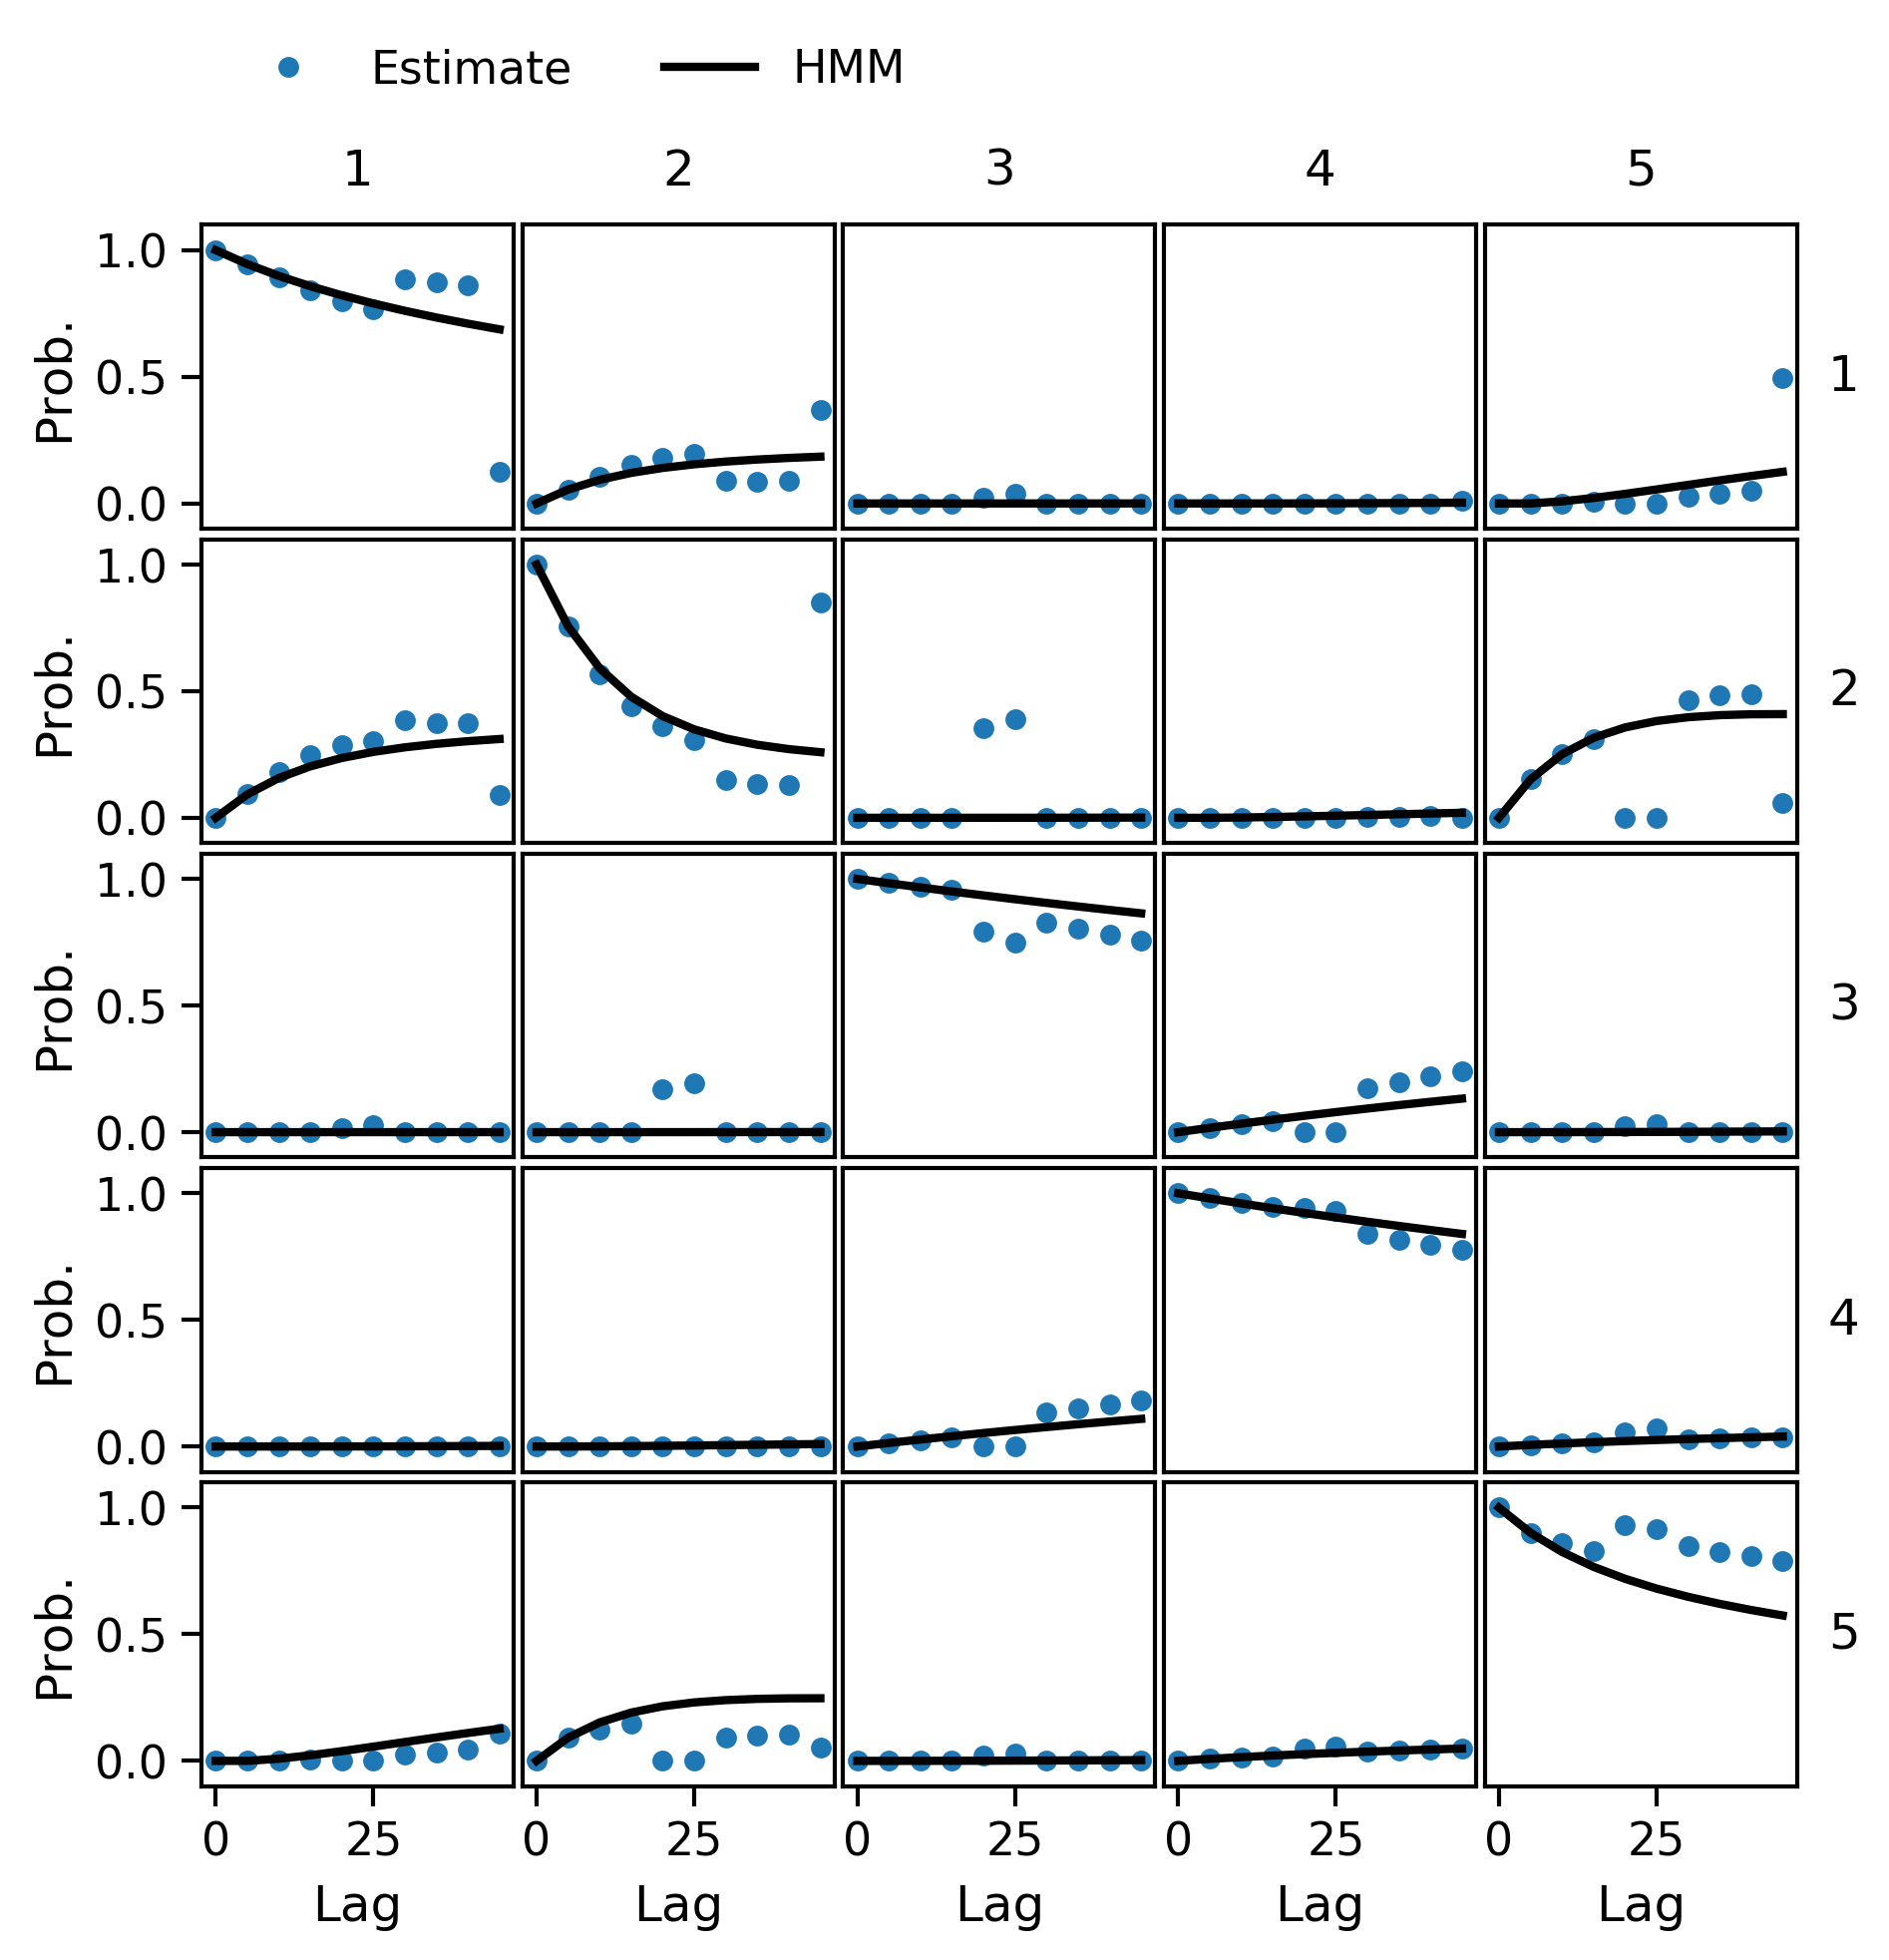
\includegraphics{chapters/hmm_selection/figures/ck_test_5_5.png}
    
    \label{fig:prinz_ck_test_5_5}
\end{figure}

\begin{figure}
    \centering
    \mycaption{CK test for Prinz Potential with $\tau=5$ and $g=9$}
    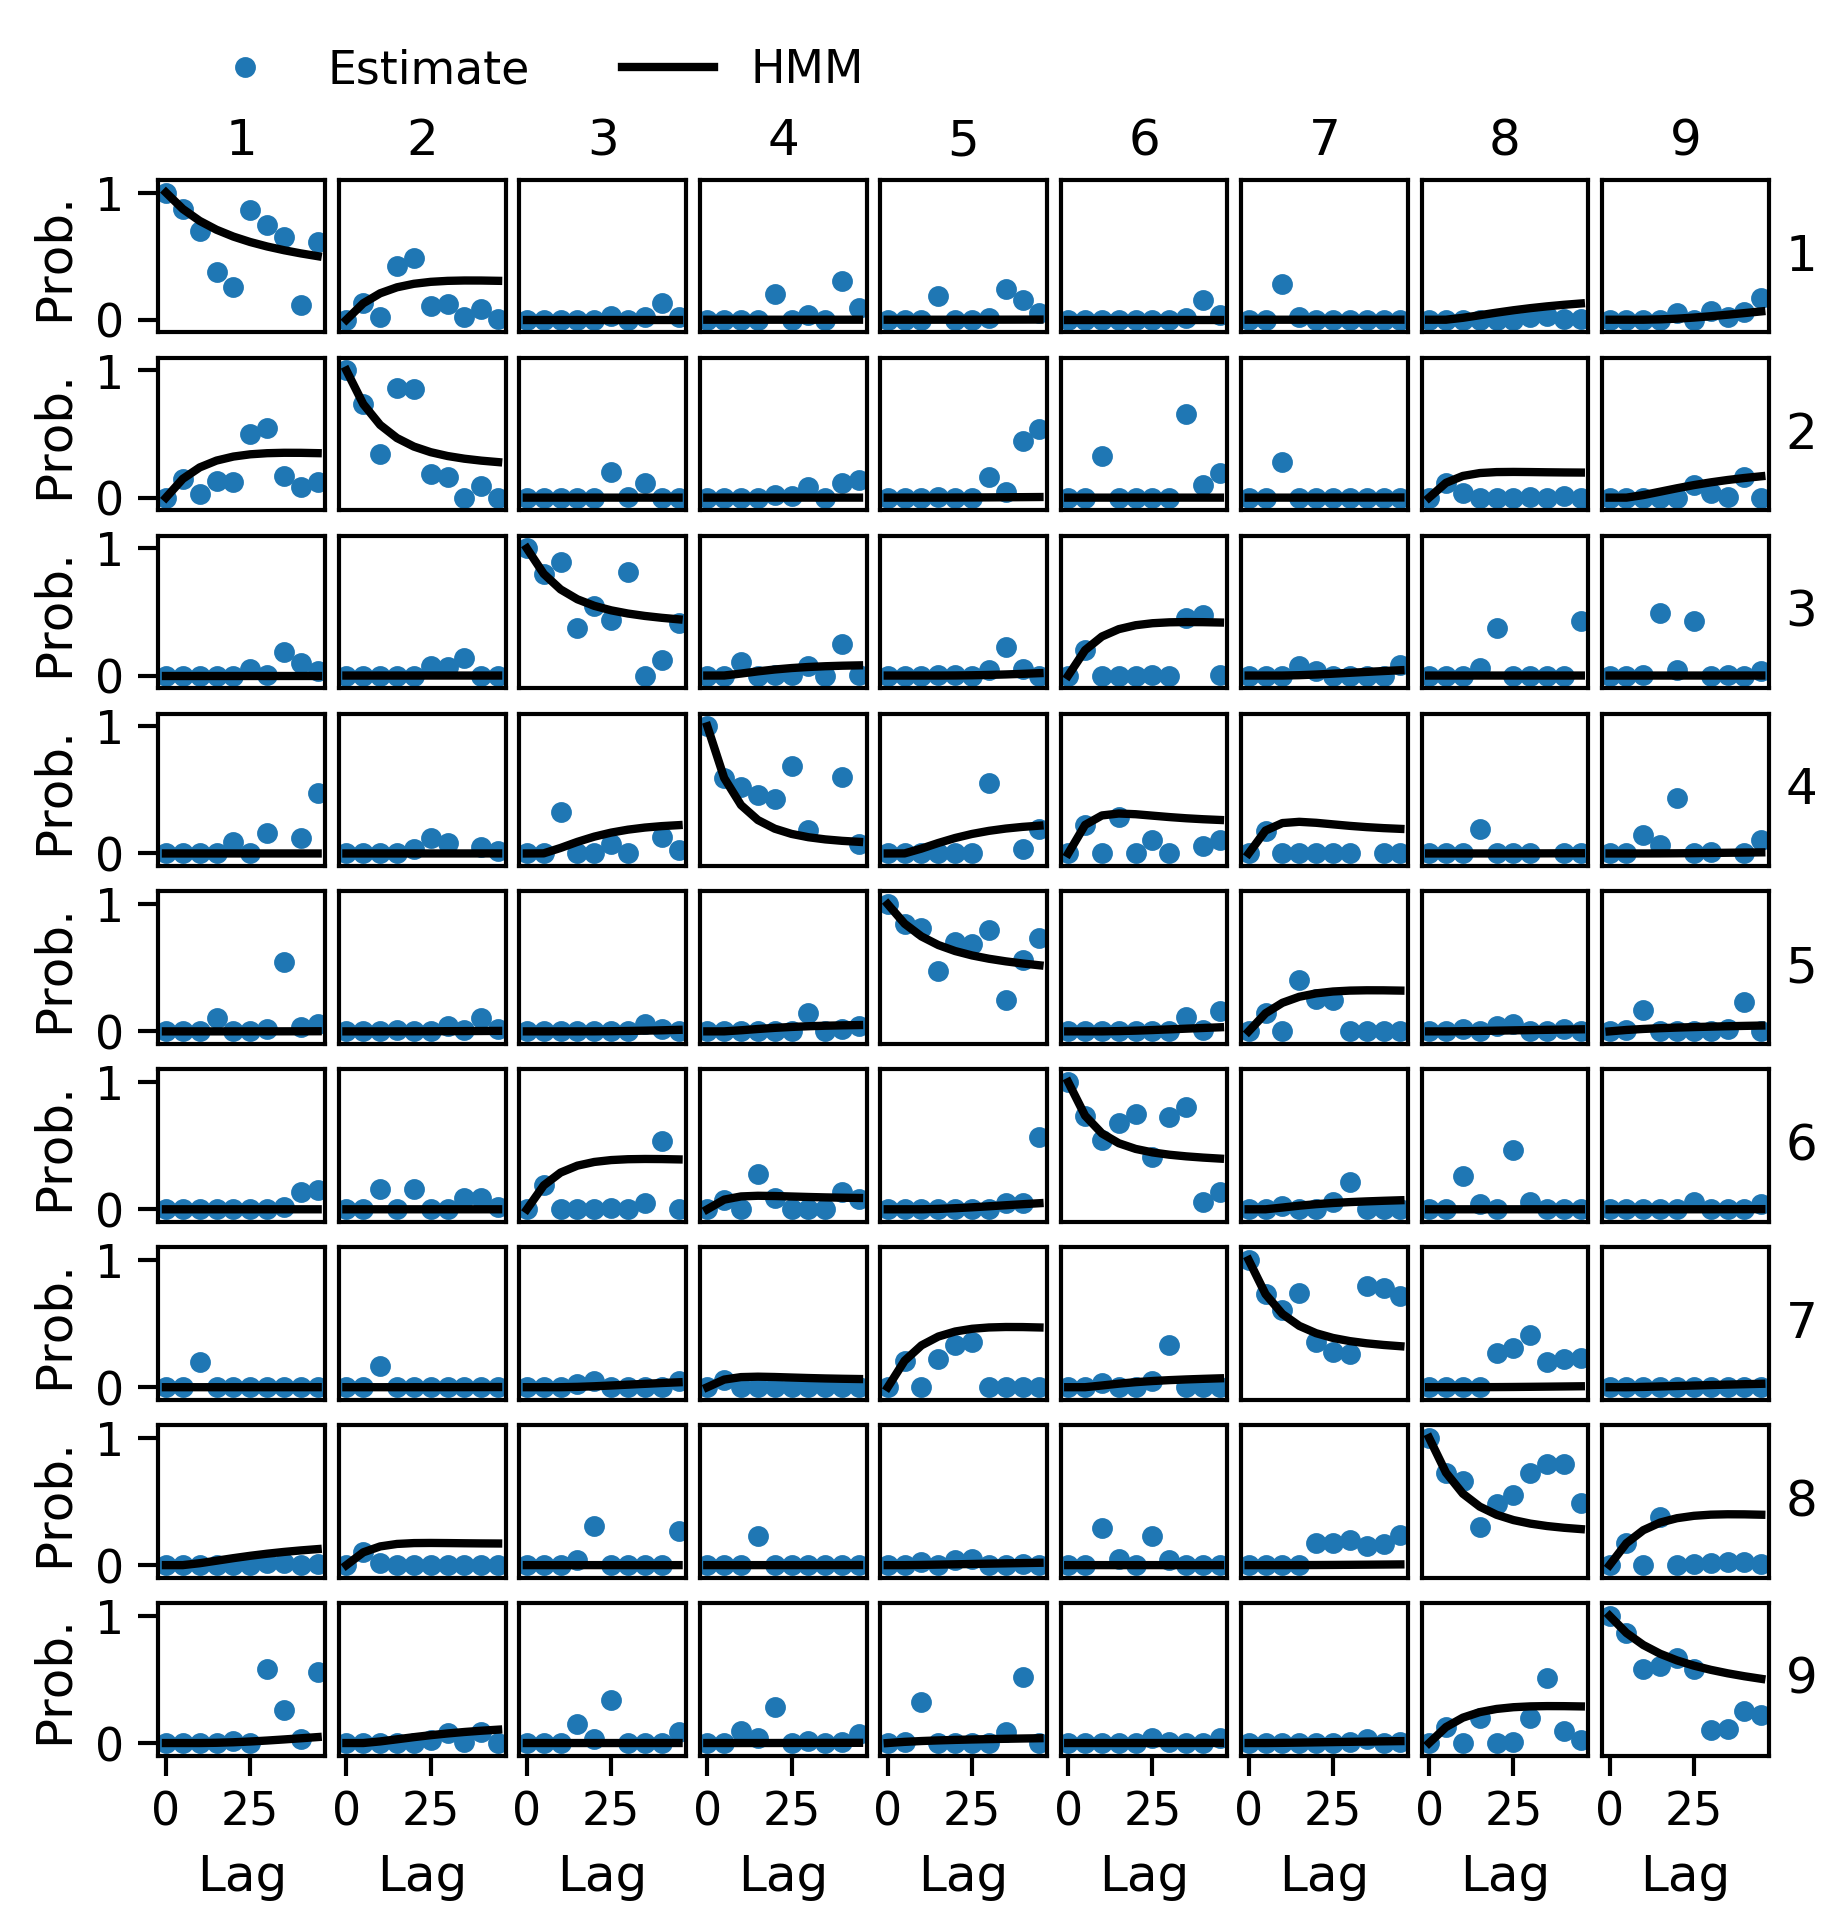
\includegraphics{chapters/hmm_selection/figures/ck_test_5_9.png}
    
    \label{fig:prinz_ck_test_5_9}
\end{figure}

\begin{figure}
    \centering
    \mycaption{CK test for Prinz Potential with $\tau=5$ and $g=10$}
    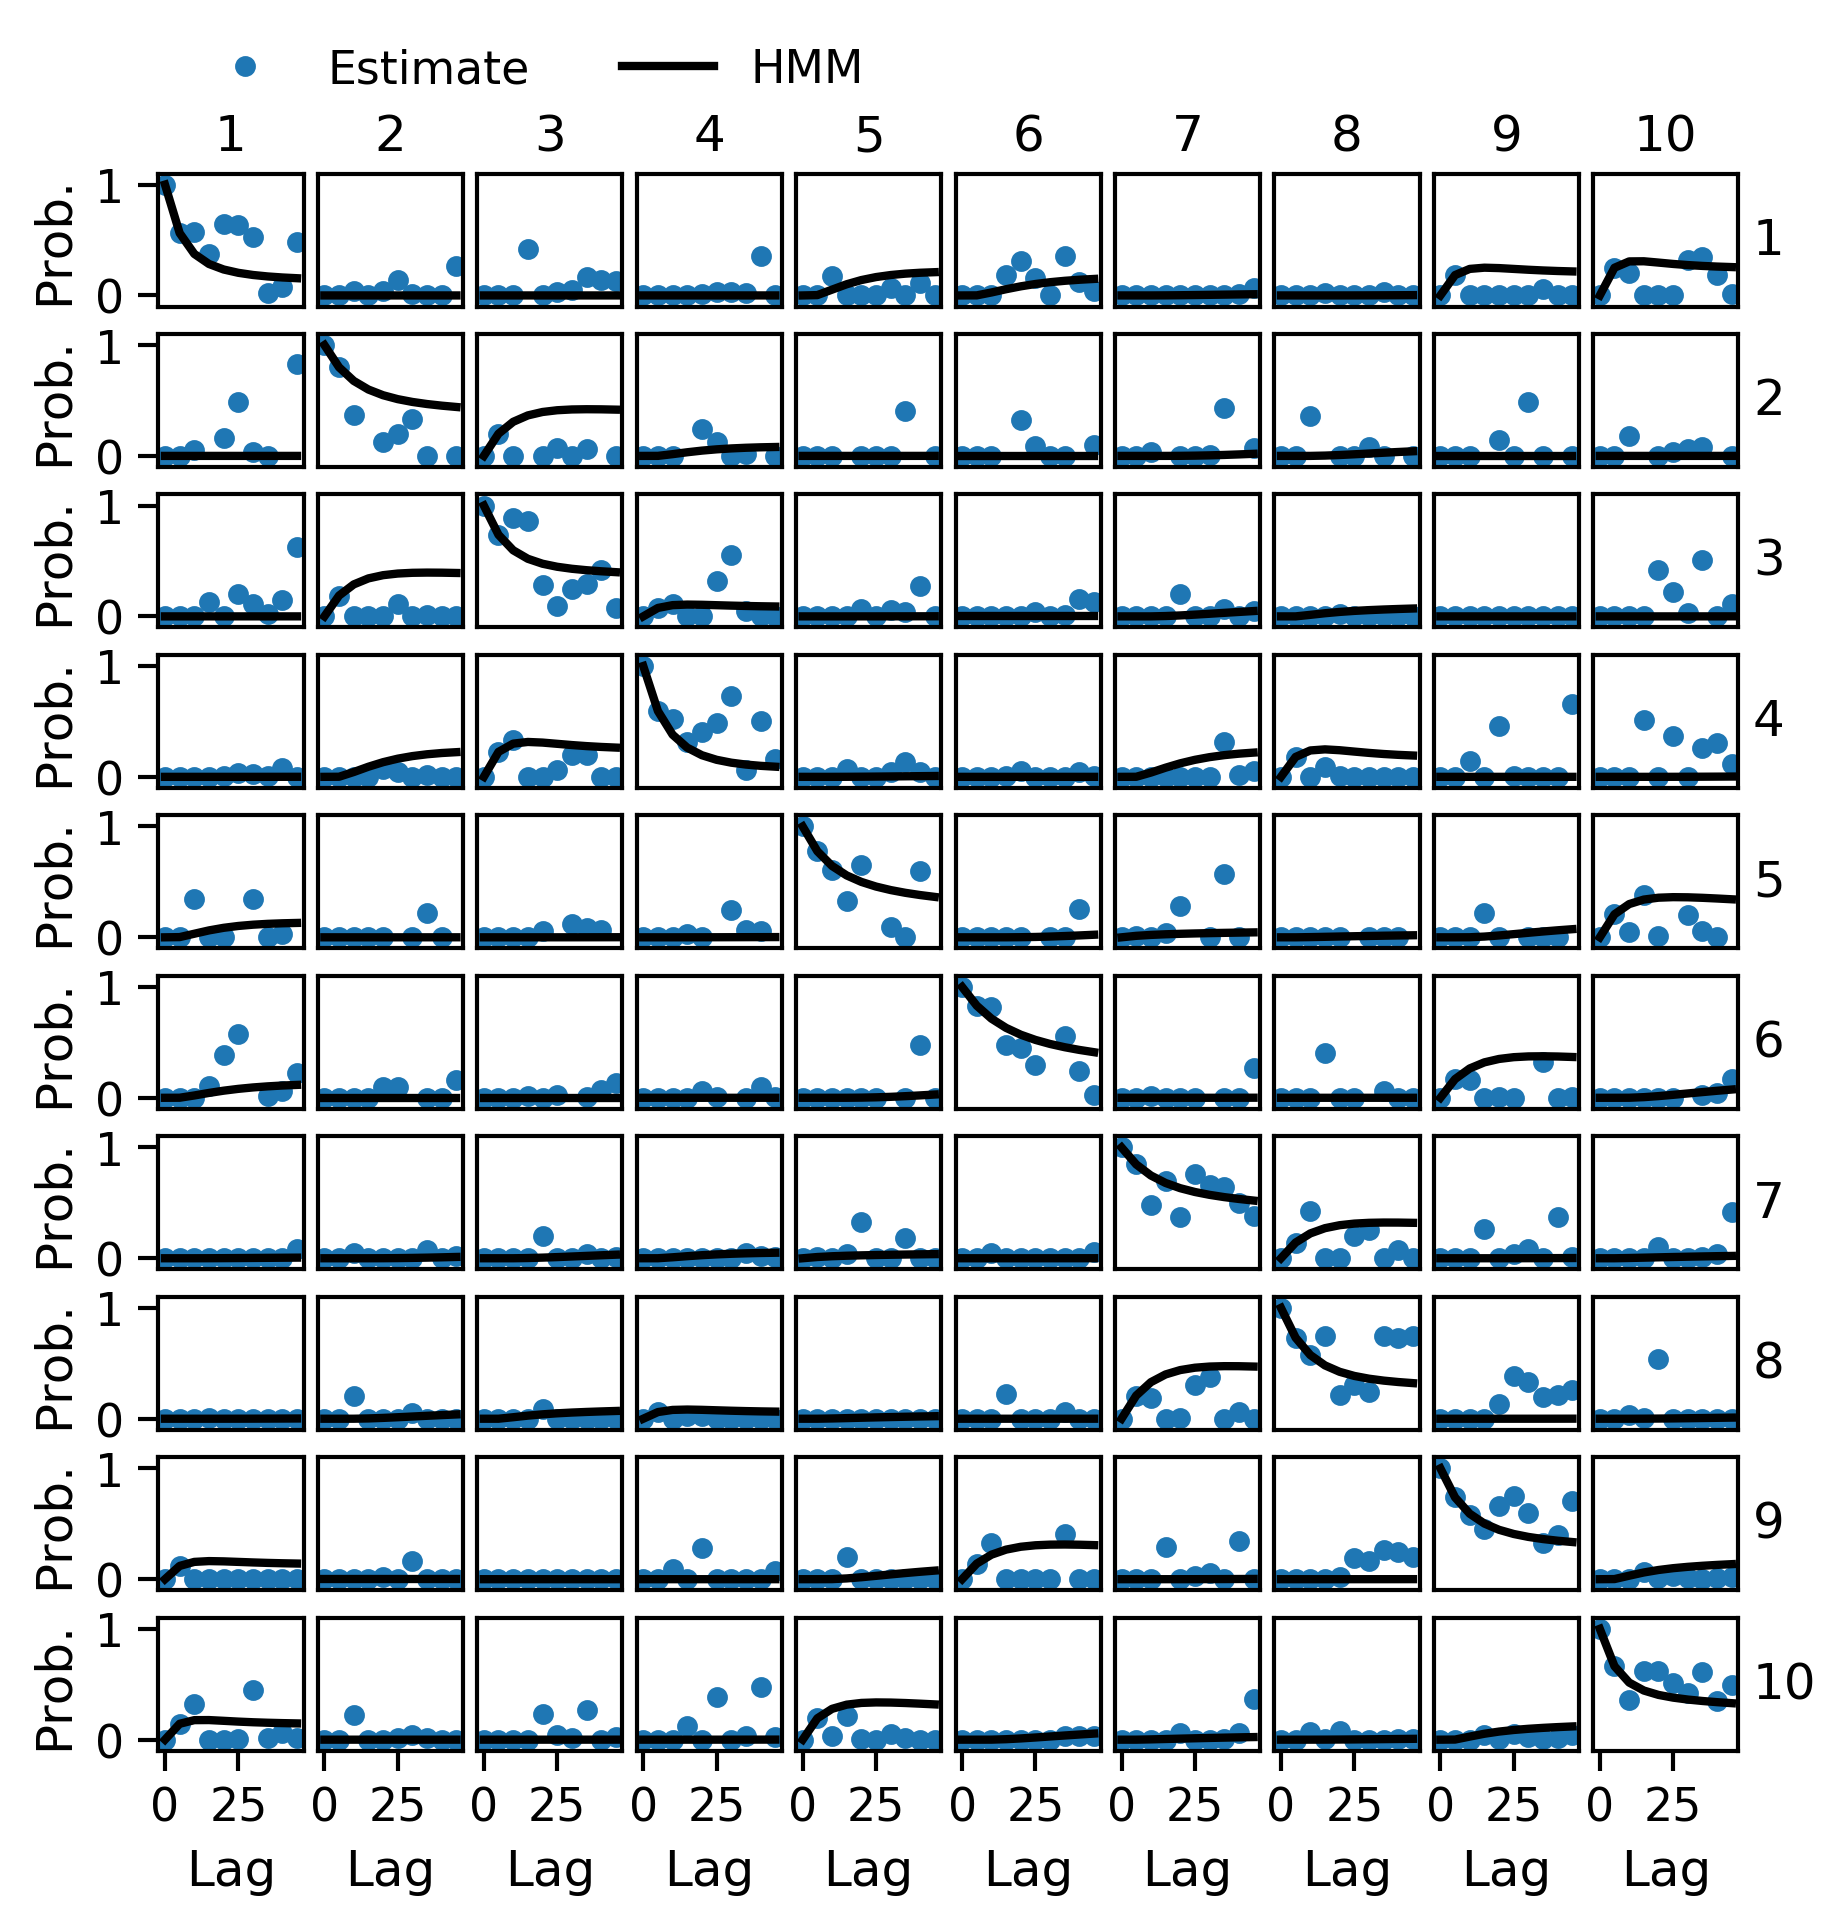
\includegraphics{chapters/hmm_selection/figures/ck_test_5_10.png}
    \label{fig:prinz_ck_test_5_10}
\end{figure}

\begin{figure}
    \centering
    \mycaption{implied timescales for $g = 2, 3, 4, 5, 9, 10$}
    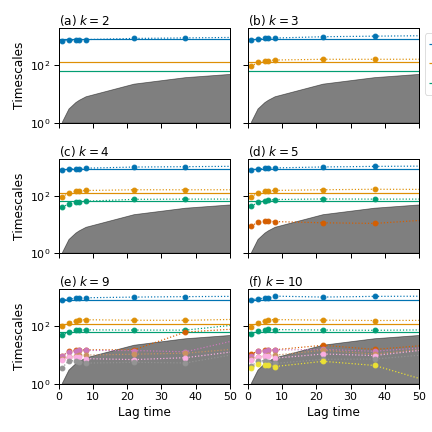
\includegraphics{chapters/hmm_selection/figures/its_tau_5.png}
    \label{fig:prinz_its_tau_5}
\end{figure}